% !TeX spellcheck = en_US
\documentclass[12pt, a4paper]{article}
\usepackage{comment}
\usepackage{ragged2e}
\usepackage{amsmath}
\usepackage{xcolor}
\usepackage{multirow}
\usepackage{caption}
\usepackage{tikz}
\usepackage{booktabs}
\usepackage{tabu}
\usepackage{placeins}
\usepackage{pdflscape}
\usetikzlibrary{arrows}
\usepackage[hidelinks]{hyperref}
\usepackage{multirow}
\usepackage{subcaption}
 \usepackage{pdflscape}


\captionsetup{font=footnotesize,labelfont=footnotesize}

%\hypersetup{
%    colorlinks=false,
%    linkcolor=False,
%    filecolor=blue,      
%    urlcolor=blue,
%    citecolor=blue
%}

\usepackage{natbib}
\usepackage[title]{appendix}

\tikzstyle{startstop} = [rectangle, rounded corners, minimum width=2cm, minimum height=0.75cm,text centered, draw=black, fill=red!30]

\tikzstyle{startstop1} = [rectangle, rounded corners, minimum width=2cm, minimum height=0.75cm,text centered, draw=black, fill=blue!30]

\tikzstyle{startstop2} = [rectangle, rounded corners, minimum width=2cm, minimum height=0.75cm,text centered, draw=black, fill=yellow!30]

\tikzstyle{startstop3} = [rectangle , rounded corners, minimum width=0.5cm, minimum height=0.75cm,text centered,draw=black]


\tikzstyle{io} = [trapezium, trapezium left angle=70, trapezium right angle=110, minimum width=2cm, minimum height=0.75cm, text centered, draw=black, fill=blue!30]



\tikzstyle{process} = [rectangle, minimum width=2cm, minimum height=1cm, text centered, draw=black, fill=green!30]

\tikzstyle{decision} = [diamond, minimum width=0.75cm, minimum height=0.75cm, text centered, draw=black, fill=green!30]

\tikzstyle{arrow} = [thick,->,>=stealth]



\def\sym#1{\ifmmode^{#1}\else\(^{#1}\)\fi}


\renewcommand{\today}{\ifcase \month \or January\or February\or March\or %
April\or May \or June\or July\or August\or September\or October\or November\or %
December\fi, \number \year} 



\def\boxit#1{%
  \smash{\color{red}\fboxrule=1pt\relax\fboxsep=2pt\relax%
  \llap{\rlap{\fbox{\vphantom{0}\makebox[#1]{}}}~}}\ignorespaces
}


\usepackage{lipsum}
\usepackage{xepersian}
\settextfont{XB Zar.ttf}
\settextdigitfont{XB Zar.ttf}
\linespread{1.2}


\title{
	اثر ساختار مالکیت و گروه های کسب و کار بر هم حرکتی سهام شرکت های بورس تهران
}
\author{
سید مرتضی آقاجان زاده امیرکلایی}

\begin{document}
\maketitle


\begin{abstract}
در این پژوهش با استفاده از داده های روزانه مالکیت  شرکت های فعال در  بورس اوراق بهادار تهران نشان می دهیم مالکیت مشترک و عضویت در یک گروه کسب و کار بر هم حرکتی قیمت شرکت ها تاثیر مثبتی دارد. علاوه بر این نشان می دهیم که عضویت در گروه کسب و کار تاثیر بیشتری از مالکیت مشترک دارد و مالکیت مشترک تنها در درون گروه های کسب و کار سبب افزایش هم حرکتی می شود.
در ادامه با توجه به شواهد معرفی شده نشان می دهیم معاملات هم زمان و هم جهت در گروه های کسب و کار هم حرکتی بیشتر شرکت ها را توضیح می دهد.
\end{abstract}




\section{Introduction}
در سال های اخیر با
\begin{itemize}
\item
هم حرکتی مورد توجه تحلیلگران بازار و محققان قرار گرفته است
\item
بعد از بحران مالی سال 2007 مدل های برآورد ریسک اهمیت پیدا کرده است
\item
در این مدل ها هم بستگی قیمت دارایی ها نقش تاثیرگذاری در برآورد ریسک دارد
\item
پاسخ سنتی به دلیل هم حرکتی بازده شرکت ها عوامل بنیادی دو شرکت بوده است  برای مثال 
 \lr{\cite{shiller1989comovements}}
 \item 
 ولی در سال های اخیر نشان داده شده است که هم حرکتی می تواند از عواملی غیر بنیادی به وجود بیاید. 
 \item
 مدل های تئوری برای  هم حرکتی میان بازده شرکت های غیر مرتبط از لحاظ بنیادی
 \lr{\cite{barberis2003style},\cite{barberis2005comovement}}
 \item
 معرفی عوامل دیگر برای هم حرکتی قیمت شرکت ها
 \begin{itemize}
 \item 
 عضو بودن شرکت ها در شاخص
  \lr{S\&P500} [\lr{\cite{barberis2005comovement}}]
      \item
      توجه سرمایه گذاران به شرکت ها
      [\lr{\cite{wu2014investor}}]  
        \item 
      پذیره نویسی توسط بانک سرمایه گذاری 
      (\lr{investment bank})
      
      [\lr{\cite{grullon2014comovement}}]  
      \item
      باور های یکسان و مرتبط
      [\lr{\cite{david2016correlated}}] 
         \item
         هم زمان بودن نیاز های نقدینگی سهامداران شرکت ها
         [\lr{\cite{pantzalis2017shareholder}}]  
            \item
         پرداخت سود تقسیمی توسط شرکت ها
         [\lr{\cite{HAMEED2019103}}]  
 \end{itemize}



\end{itemize}

\begin{itemize}
\item 
از طرف دیگر در سال های اخیر مسئله مالکیت مشترک ادبیات مالی مورد توجه قرار گرفته است
\footnote{
	با توجه به افزایش صندوق های سرمایه گذاری  دنبال کننده شاخص در آمریکا، مسئله مالکیت مشترک در میان شرکت های آمریکا افزایش داشته است و این امر سبب شده است که در ادبیات مسئله بررسی مالکیت مشترک و عملکرد شرکت ها و همچنین رفتار بازده ای شرکت ها مورد توجه قرار گیرد. 
	برای مثال 
	\lr{\cite{azar2018anticompetitive}}
	با افزایش مالکیت مشترک میان شرکت های هواپیمایی رقابت قیمتی شرکت ها کاهش پیدا می کند.  اما در این رابطه بحث و گفت و گو همچنان ادامه دارد و مقالات زیادی در رد و تایید اثر مالکیت مشترک بر روی رفتار شرکت ها وجود دارد. برای مثال مقاله
	\lr{\cite{lewellen2021does}}
	مقالات سال های گذشته را بررسی کرده است و یافته است که در بررسی های گذشته، اثر دیگر فاکتور های تاثیر گذار به اشتباه به مالکیت مشترک مرتبط شده است.
}
 و
\lr{\cite{AntonPolk}}
اثر مالکیت مشترک را بر هم حرکتی را بررسی کرده است.  

\begin{itemize}
\item \lr{\cite{AntonPolk}}
\begin{itemize}
\item
یافته است که با افزایش مالکیت مشترک هم حرکتی شرکت ها افزایش پیدا می کند. 
%\item
%علاوه بر این با توجه به دسترسی به داده های مالکیت صندوق های سرمایه گذاری مقاله نشان داده است که هم حرکتی شرکت ها هنگامی که جریان خروجی و ورودی قوی ای در صندوق ها وجود داشته باشد افزایش پیدا می کند. 
\item
این مقاله بررسی خود را محدود به صندوق های سرمایه گذاری فعال 
(\lr{Active mutual funds}) 
و شرکت های بزرگ (ارزش بازاری بالاتر از میانه ارزش شرکت ها) محدود کرده است.
\end{itemize}
\end{itemize}
\item
در ادامه 
\lr{\cite{Liquidity2016}}
نشان داده است که شرکت ها با توجه به هم بستگی نیاز های نقدینگی مالکان خود، با یکدیگر هم حرکتی نشان می دهند
\begin{itemize}
\item \lr{\cite{Liquidity2016}}:
\begin{itemize} 
\item
 نشان می دهد که شرکت های دارای سطح بالایی از مالکیت صندوق های سرمایه گذاری همراهی نقدشوندگی بالاتری نسبت به بقیه شرکت ها دارند.
 \item
 نشان می دهد که برای هم حرکتی قیمت شرکت ها نیاز به مالکیت مشترک نیست
 \item
 همچنین نشان می دهد که مالکیت مشترک می تواند هم بستگی در نقد شوندگی سهام شرکت را توضیح دهد
\end{itemize}

\item
نتایج به دست آمده در پژوهش های قبلی با استفاده از داده های مالکیت صندوق های سرمایه گذاری بدست آمده است
\item
در نتیجه نتایج بدست آمده محدود به این نوع مالکیت می باشد
\item
در صورتی که این نوع به خصوص مالکیت با توجه به نیاز ها و واسطه بودن، رفتار های به خصوصی انجام می دهند
\footnote{\lr{\cite{coval2007asset}} 
	نشان داده است که جریان ورود و خروج مالی صندوق ها می تواند سبب ایجاد فشار قیمتی بر سهام شرکت ها شود و قیمت شرکت ها رو تحت تاثیر قرار دهد و این مسئله با موصوع مالکیت مشترک که می تواند سبب تغییر رفتار مدیران شرکت شود می تواند متفاوت باشد.}

\end{itemize}

\item 
از طرفی دیگر 
یکی دیگر از ویژگی های بازار سرمایه ایران وجود گروه های کسب و کار است. گروه های کسب و کار حدود 85\% از ارزش بازار ایران را در اختیار دارند.
\begin{itemize}
	\item
	گروه های کسب و کار پدیده مهمی هستند در کشور های در حال توسعه یافته و در حال توسعه وجود دارند.
	\item
	هم حرکتی شرکت ها را در گروه های کسب و کار بررسی می کنیم
	\item
	دو مقاله در ادبیات به این موضوع پرداخته اند و هم حرکتی قیمت شرکت ها در گروه های کسب و کار را بررسی کرده اند
	\item
	هم حرکتی قیمت شرکت ها در گروه های کسب و کار تایید شده است ولی کانال این هم حرکتی مشخص نشده است
	\begin{itemize}
		\item \lr{\cite{cho2015stock},\cite{kim2015stock}}:
		\begin{itemize}
			دو پاسخ متفاوت به دلایل هم حرکتی شرکت ها در گروه های کسب و کار داده اند. هر دو گروه های کسب و کار موجود در بازار کره جنوبی را بررسی کرده اند و مقاله اول عوامل بنیادی مرتبط شرکت ها در گروه های کسب و کار را به عنوان دلیل هم حرکتی شرکت ها معرفی کرده است ولی مقاله دوم دسته بندی شرکت های عضو گروه را به عنوان دلیل هم حرکتی بیان کرده است. 
		\end{itemize}
		
	\end{itemize}

\end{itemize}
\item
در این بستر می توان اثر مالکیت مشترک مستقیم و غیر مستقیم را بررسی کرد
\end{itemize}

%%%% Our work
\begin{itemize}
\item 
در این پژوهش 
\item
اولین بررسی هم حرکتی ناشی از مالکیت مشترک صرف نظر از اینکه مالک شرکت صندوق سرمایه گذاری بوده باشد

\item 
در ایران داده های مالکیت های بالای یک درصد به صورت روزانه وجود دارد که محدود به مالکیت صندوق های سرمایه گذاری نیست.
\item
می توان به این سوال پاسخ داد که مالکیت مشترک فارغ از نوع مالکان سبب هم حرکتی می شود و یا خیر
\end{itemize}

%با توجه به محدودیت های دیتای موجود در آمریکا و  تنها موجود بودن داده های مالکیت های صندوق های سرمایه گذاری، بخشی از بررسی های این حوزه محدود به اثر مالکیت صندوق های سرمایه گذاری بر شرکت ها می باشد. برای مثال مقاله 
%\lr{\cite{coval2007asset}} 
%نشان داده است که جریان ورود و خروج مالی صندوق ها می تواند سبب ایجاد فشار قیمتی بر سهام شرکت ها شود و قیمت شرکت ها رو تحت تاثیر قرار دهد و این مسئله با موصوع مالکیت مشترک که می تواند سبب تغییر رفتار مدیران شرکت شود می تواند متفاوت باشد.


%در ایران با توجه به دسترسی به داده های مالکیت های بالای یک درصد شرکت ها به صورت روزانه، می توان با دقتی بالاتر و مشخص تر اثر مالکیت مشترک را بر روی شرکت های ثبت شده در بازار بورس مشخص کرد.  از طرف دیگر یکی دیگر از ویژگی های بازار سرمایه ایران وجود گروه های کسب و کار است. گروه های کسب و کار حدود 85\% از ارزش بازار ایران را در اختیار دارند.  در بازار های در حال توسعه در اکثر نقاط دنیا و حتی بعضی از کشرو های توسعه یافته نیز گروه های کسب و کار وجود دارند. گروه های کسب و کار مجموعه از شرکت های مرتبط با یکدیگر هستند که دارای مالک نهایی یکسان می باشند. در ادبیات موارد متعددی در رابطه با تاثیر گروه های کسب و کار بر روی شرکت ها معرفی  شده است. در رابطه با بررسی هم حرکتی در شرکت ها دو مقاله 
%\lr{\cite{cho2015stock},\cite{kim2015stock}}
%این موضوع را بررسی کرده اند و دو پاسخ متفاوت به دلایل هم حرکتی شرکت ها در گروه های کسب و کار داده اندد. هر دو گروه های کسب و کار موجود در بازار کره جنوبی را بررسی کرده اند و مقاله اول مسائل بنیادی مرتبط شرکت ها در گروه های کسب و کار را به عنوان دلیل هم حرکتی شرکت ها معرفی کرده است ولی مقاله دوم دسته بندی شرکت های عضو گروه را به عنوان دلیل هم حرکتی بیان کرده است.


\begin{itemize}
\item
در این مقاله سعی شده است تا هم حرکتی میان شرکت های درون گروه های کسب و کار بررسی شود.

\item 
و برای اولین میان مالکیت مشترک مستفیم و مالکیت مشترک غیر مستقیم مقایسه انجام شود

\end{itemize}
 
 
 \begin{itemize}
 \item
برای محاسبه مالکیت مشترک میان شرکت ها از ملاکی اصلاح شده استفاده کرده ایم که در این پژوهش معرفی کرده ایم

 \end{itemize}


\begin{itemize}
\item
مالکیت مشترک برای پیش بینی هم حرکتی قیمت شرکت ها اهمیت دارد
\item 
گروه های کسب و کار برای پیش بینی هم حرکتی قیمت شرکت ها اهمیت دارد
\item
اهمیت گروه های کسب و کار برای پیش بینی هم حرکتی قیمت شرکت ها بیشتر از مالکیت مشترک است
\item
 در گروه های کسب و کار، مالکیت مشترک سبب افزایش هم حرکتی قیمت می شود ولی در خارج از گروه های کسب و کار اهمیت ندارد
\end{itemize}



\begin{itemize}
\item 
انواع بررسی ها برای تایید اهمیت گروه های کسب و کار انجام شده است 
\begin{itemize}

\item
فقط جفت  های د ارای مالکیت بالا را بررسی کردیم
\begin{itemize}
\item 
در این زیر مجموعه هم گروه های کسب و کار بیشترین تاثیر را دارند 
\item
مالکیت مشترک صرفا در گروه های کسب و کار اهمیت دارند.

\end{itemize}
\item
بررسی ها محدود به جفت های دارای مالک مشترک بوده است:
\begin{itemize}
\item
بررسی اثر گروه کسب و کار نیاز به مالکیت مشترک ندارد
\item
اثر گروه کسب و کار و مالکیت مشترک را نمی توان جدا کرد
\item 
همه ی جفت های بازار را ساختیم و اهمیت گروه ها کسب و کار نسبت به مالکیت مشترک مستقیم تایید شده است.
%\begin{itemize}
%\item
%نتایج اولیه تایید شد
%\item 
%جفت های حاضر در گروه های کسب و کار سطح مالکیت مشترک اهمیت ندارد و صرفا سطح بالایی از مالکیت مشترک اهمیت دارد
%\item
%برای جفت های بیرون یک گروه کسب وکار، سطح مالکیت در واقع وجود مالکیت مشترک اهمیت دارد و نه مقدار قابل توجه آن
%\item
%مالکیت مشترک خارج از گروه های کسب و کار نیز اهمیت دارد
%\item
%تاثیر یکسان بودن گروه های کسب و کار بیشتر است
%\end{itemize}
\end{itemize}

\end{itemize}


	\item
کانال تاثیر: معامله هم زمان شرکت ها با یکدیگر در گروه های کسب و کار
\begin{itemize}

	\item
	از دو پراکسی برای بررسی اثر معاملات هم زمان در گروه های کسب و کار 
	\item
	\lr{turnover} 
	و ناترازی خرید و فروش حقوقی استفاده کرده ایم
	\item
	پراکسی اول معاملات هم زمان را تایید می کند
	\item
	پراکسی دوم هم جهتی معاملات را تایید می کند
	%\begin{itemize}
	%\item
	%\lr{turnover}
	%\begin{itemize}
	%\item
	%بخش قابل توجهی از تغییرات 
	%\lr{turnover}
	%شرکت ها علاوه بر بازار از گروه های کسب و کار ناشی می شود
	%\item
	%حضور شرکت ها در گروه های کسی و کار می تواند هم بستگی 
	%\lr{turnover}
	%را توضیح دهد.
	%\item
	%از 
	%\lr{turnover}
	%ماهانه شرکت ها 
	%میانگین 
	%\lr{turnover}
	%سالانه شرکت و 
	%\lr{turnover}
	%ماهانه بازار را خارج کردیم و بررسی کردیم درگروه های کسب و کار میزان پراکندگی باقی مانده ماهانه کمتر است
	%\item
	%برای گروه های با پراکندگی کمتر هم حرکتی بیشتر است
	%
	%% گروه های کسب و کار بزرگ
	%% \begin{itemize}
		%% 	\item 
		%% 	اگر معامله گران شرکت های در یک گروه کسب و کار را در یک دسته قرار می دهند نیاز است تا اعضای گروه های بزرگ هم حرکتی بیشتری داشته باشند
		%% 	\item
		%% 	علاوه بر مورد فوق باید رابطه هم بستگی 
		%% 	\lr{turnover}
		%% 	و هم حرکتی بازده نیز مثبت باشد. 
		%% 	
		%% 		\item 
		%% 		شرکت های عضو گروه کسب و کار به همراه یکدیگر معامله بشوند
		%% 		
		%% 	
		%% \item
		%% بررسی کردیم و نتایج نشان داد که شرکت های در گروه بزرگ هم حرکتی بیشتری دارند و علاوه بر این تاثیر هم حرکتی در 
		%% \lr{turnover}
		%% نیز در گروه های بزرگ از دیگر گروه ها بیشتر است.
		%% \end{itemize}
	%\end{itemize}
	%\item 
	%ناترازی خرید حقوقی
	%\begin{itemize}
	\item
	پراکندگی ناترازی خرید و فروش حقوقی در این شرکت ها باید کم باشد
	\item 
	به صورت کلی در گروه های کسب و کار میانگین پراکندگی شاخص ناترازی کمتر از شرکت های بیرون گروه است
	\item
	بررسی دقیق تر نشان داد با مشخص کردن گروه های کسب و کار دارای پراکندگی کم انتظار داریم با کاهش پراکندگی، هم حرکتی افزایش پیدا کند
	\item
	در گروه های با پراکندگی کم، هم حرکتی شرکت ها افزایش پیدا می کند و با افزایش مالکیت مشترک نیز هم حرکتی افزایش پیدا می کند
	
	\item
	کانال عوامل بنیادی را بررسی کردیم ولی تاثیری بر هم حرکتی قیمت ها یافت نشد
	
\end{itemize}



\end{itemize}







\section{داده و روش شناسی}



\subsection{داده}
\begin{itemize}
	\item 
	داده های قیمت، حجم و دیگر مشخصات حسابداری و بازاری شرکت ها از سایت کدال و tsetmc
	\item
	داده منحصر به فرد مالکیت های بالای یک درصد روزانه شرکت ها بورسی از سایت 
	tsetmc
	\item 
	حذف داده های صندوق های سرمایه گذاری معامله پذیر
	\item 
	از تاریخ 
	1393/01 (2014/03)
	 تا تاریخ 
	 1398/12 (2020/03)
	 

	\item 
	گروه های کسب و کار یکی از مشخصات بازار ایران است
		\item 
	داده های گروه های کسب و کار از مقاله
	\lr{\cite{Aliabadi2022}}
	\begin{itemize}
		\item 
		داده های گروه های کسب و کار در ایران مشخص نیست
		\item
		با استفاده از الگوریتم 
		\lr{\cite{almeida2011structure}}
		با آستانه 40\%
		
	\end{itemize}
	\item
	جدول 
	\ref{t2-1}
	مشخصات آماری داده های مالکیت
\end{itemize}
%داده های مالکیت، قیمت، حجم و دیگر متغیر های بازاری و حساب داری شرکت ها از سایت کدال و شركت مديريت فناوري بورس تهران جمع آوری شده است. علاوه بر این به داده های منحصر به فرد 


\begin{LTR}
\lr{	 \begin{table}[htbp]
        \centering
        \caption{ This table reports summary statistics of ownership features for all the listed firms. At this table by group, we mean business groups.}
        \label{t2-1}
        \resizebox{1\textwidth}{!}
        {
        \begin{tabular}{lrrrrrr}
\toprule
Year &  2014 &  2015 &  2016 &  2017 &  2018 &  2019 \\
\midrule
No. of Firms                        &   365 &   376 &   446 &   552 &   587 &   618 \\
No. of Blockholders                 &  1606 &  1676 &  2099 &  2978 &  3374 &  3416 \\
No. of Groups                       &    38 &    41 &    43 &    44 &    40 &    43 \\
No. of Firms in Groups              &   249 &   268 &   300 &   336 &   346 &   375 \\
Ave. Number of group Members        &     7 &     7 &     7 &     8 &     9 &     9 \\
Ave. ownership of each Blockholders &    18 &    19 &    18 &    17 &    18 &    19 \\
Med. ownership of each Blockholders &     5 &     4 &     4 &     4 &     4 &     4 \\
Ave. Number of Owners               &     7 &     6 &     6 &     7 &     7 &     7 \\
Ave. Block. Ownership               &    77 &    77 &    75 &    76 &    75 &    72 \\
\bottomrule
\end{tabular}

         }
      \end{table}}
\end{LTR}



\subsection{\lr{Pair composition} }
\begin{itemize}
	\item 
	حداقل یک مالک مشترک که 
		\item 
		612 شرکت حداقل یک مالک مشترک با دیگر شرکت ها داشتند
	\item 
	93442 جفت که 25 درصد از جفت های ممکن
	$ (612*611)/2 = 373932$

	\item 
	جدول
	 \ref{t2-2}
	 خلاصه آماری جفت های تشکیل شده
	\item 
	برای قرار گرفتن شرکت ها در گروه های کسب و کار 
	\begin{itemize}
		\item
		 چند حالت امکان دارد 
		 \item
		 در شکل 
		 \ref{g2-1}
		 حالت های مختلف بیان شده است
	\end{itemize}
	
\end{itemize}

 
\begin{LTR}
	\lr{  \begin{table}
  \centering
  \caption{ This table reports summary statistics of ownership features for total pairs. At this table by group, we mean business groups.}
  \label{t2-2}
    \resizebox{1\textwidth}{!}
          {
 \begin{tabular}{lrrrrrr}
\toprule
year &   1393 &   1394 &   1395 &   1396 &   1397 &   1398 \\
\midrule
No. of Pairs                          &  20876 &  21187 &  27784 &  41449 &  47234 &  67232 \\
No. of Groups                         &     37 &     40 &     42 &     43 &     39 &     43 \\
No. of Pairs not in Groups            &  11452 &  11192 &  15351 &  26530 &  29182 &  43433 \\
Number of Pairs not in the same Group &   7962 &   8731 &  10971 &  12916 &  15366 &  20745 \\
Number of Pairs in the same Group     &    923 &    955 &   1099 &   1260 &   1536 &   1774 \\
Average Number of Common owner        &      1 &      1 &      1 &      1 &      1 &      1 \\
Med. Number of Common owner           &      1 &      1 &      1 &      1 &      1 &      1 \\
Average Percent of each blockholder   &     19 &     19 &     19 &     19 &     19 &     20 \\
Med. Percent of each blockholder      &     13 &     12 &     12 &     12 &     12 &     14 \\
Average Number of Pairs in one Group  &     31 &     30 &     30 &     34 &     39 &     44 \\
Med. Number of Pairs in one Group     &      8 &     10 &      8 &     10 &      9 &     10 \\
Average Number of Owners              &      5 &      5 &      5 &      5 &      4 &      5 \\
Med. Number of Owners                 &      5 &      5 &      5 &      5 &      4 &      5 \\
Average Block. Ownership              &     73 &     73 &     72 &     70 &     70 &     70 \\
Med. Block. Ownership                 &     73 &     73 &     73 &     71 &     71 &     71 \\
\bottomrule
\end{tabular}

   }
    \end{table} }
\end{LTR}

\begin{figure}[htbp]
	\centering
	\caption{ \lr{Three categories for pairs base on being in business groups}}
	\label{g2-1}
	
	\normalcolor
	\begin{subfigure}[t]{0.9\linewidth}
		
		\resizebox{0.49\textwidth}{!}{
			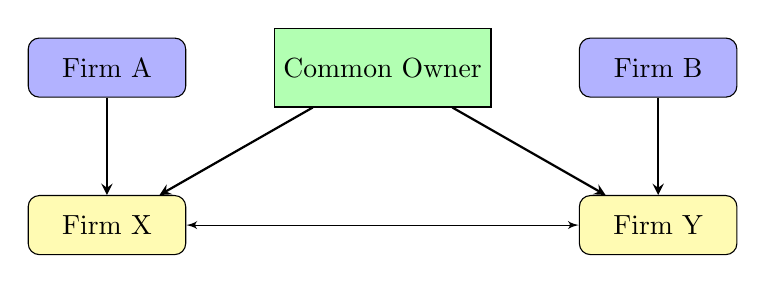
\begin{tikzpicture}[node distance=2cm]
				
				
				
				\node (CH) [process,yshift = -2cm ,xshift=3.5cm] {Common Owner};
				
				\node (end) [startstop1,left of = CH ,xshift=-1.5cm ] {$ \text{Firm A} $};
				
				\node (end2) [startstop1,right of = CH ,yshift=0cm,xshift=1.5cm] {$ \text{Firm B} $};
				
				\node (sur) [startstop2 ,below of = end ,yshift=0cm,xshift=0cm] {$ \text{Firm X} $};
				
				\node (sur2) [startstop2,below of = end2 ,yshift=0cm,xshift=0cm] {$ \text{Firm Y} $};
				
				
				\draw [arrow] (end) --(sur);
				\draw [arrow] (end2) -- (sur2);
				
				
				\draw [arrow] (CH) -- (sur);
				\draw [arrow] (CH) -- (sur2);
				
				\draw [latex'-latex'] (sur) to [bend right =0]  node[sloped, anchor=center, below] {} (sur2);
				
				
			\end{tikzpicture}
		}   
		\hfill
		\resizebox{0.49\textwidth}{!}{
			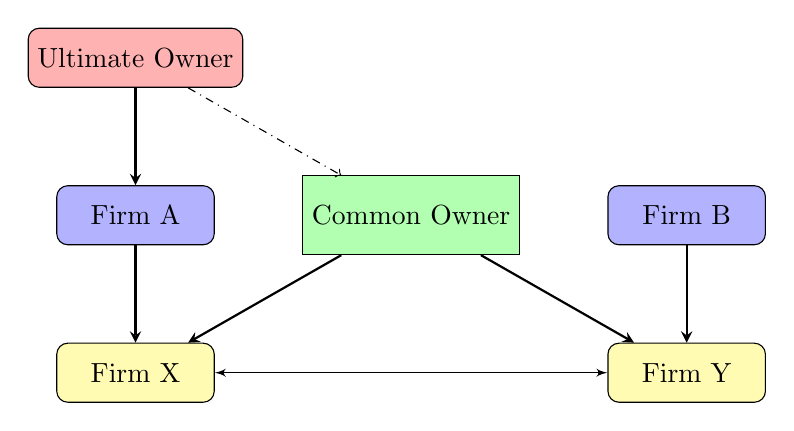
\begin{tikzpicture}[node distance=2cm]
				
				
				\node (start) [startstop] { $ \text{Ultimate Owner} $};
				
				
				\node (CH) [process, below of = start,xshift=3.5cm] {Common Owner};
				
				\node (end) [startstop1,below of = start ] {$ \text{Firm A} $};
				
				\node (end2) [startstop1,right of = CH ,yshift=0cm,xshift=1.5cm] {$ \text{Firm B} $};
				
				\node (sur) [startstop2 ,below of = end ,yshift=0cm,xshift=0cm] {$ \text{Firm X} $};
				
				\node (sur2) [startstop2,below of = end2 ,yshift=0cm,xshift=0cm] {$ \text{Firm Y} $};
				
				
				
				\draw [arrow] (start) --(end);
				
				\draw [arrow] (end) --(sur);
				\draw [arrow] (end2) -- (sur2);
				
				\draw [dash dot,->] (start) -- (CH);
				
				\draw [arrow] (CH) -- (sur);
				\draw [arrow] (CH) -- (sur2);
				
				\draw [latex'-latex'] (sur) to [bend right =0]  node[sloped, anchor=center, below] {} (sur2);
				
				
			\end{tikzpicture}
		}
		\caption{ \lr{Pair not in the business group}}
	\end{subfigure}
	\bigskip
	\begin{subfigure}[t]{.45\linewidth}
		\centering
		\tiny
		\resizebox{1\textwidth}{!}{
			
			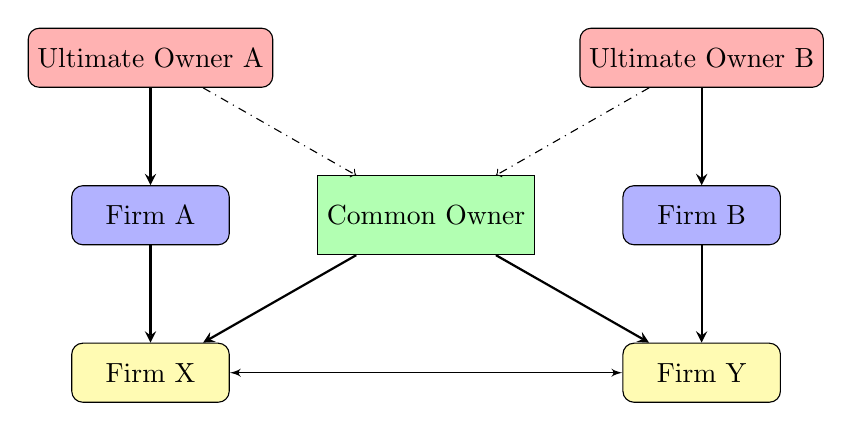
\begin{tikzpicture}[node distance=2cm]
				
				
				\node (start) [startstop] { $ \text{Ultimate Owner A} $};
				\node (start2) [startstop,right of = start,xshift=5cm] {$ \text{Ultimate Owner B} $};
				
				
				\node (CH) [process, below of = start2,xshift=-3.5cm] {Common Owner};
				
				\node (end) [startstop1,below of = start ] {$ \text{Firm A} $};
				
				\node (end2) [startstop1,below of = start2 ,yshift=0cm,xshift=0cm] {$ \text{Firm B} $};
				
				\node (sur) [startstop2 ,below of = end ,yshift=0cm,xshift=0cm] {$ \text{Firm X} $};
				
				\node (sur2) [startstop2,below of = end2 ,yshift=0cm,xshift=0cm] {$ \text{Firm Y} $};
				
				
				
				\draw [arrow] (start) --(end);
				\draw [arrow] (start2) -- (end2);
				
				\draw [arrow] (end) --(sur);
				\draw [arrow] (end2) -- (sur2);
				
				\draw [dash dot,->] (start) -- (CH);
				\draw [dash dot,->] (start2) -- (CH);
				
				\draw [arrow] (CH) -- (sur);
				\draw [arrow] (CH) -- (sur2);
				
				\draw [latex'-latex'] (sur) to [bend right =0]  node[sloped, anchor=center, below] {} (sur2);
				
				
			\end{tikzpicture}
		}   
		\caption{\lr{ Pair in two distinct business group}}
	\end{subfigure}
	\begin{subfigure}[t]{.45\linewidth}
		\centering
		\tiny
		\resizebox{1\textwidth}{!}{
			
			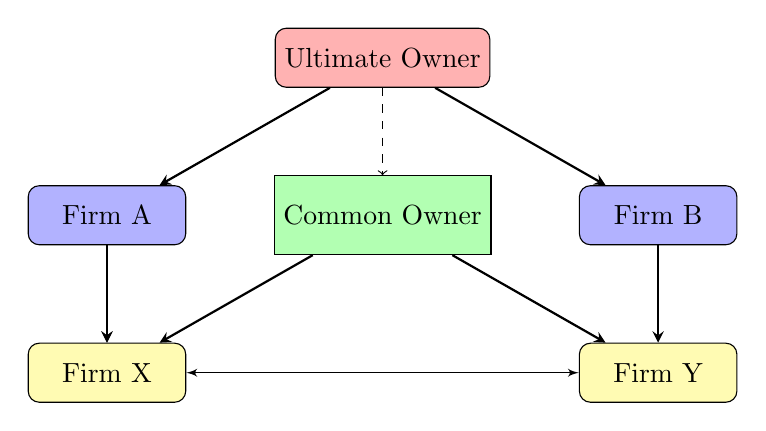
\begin{tikzpicture}[node distance=2cm]
				
				
				\node (start) [startstop] {Ultimate Owner};
				
				
				
				\node (end) [startstop1,below of = start , yshift=0cm , xshift=-3.5cm ] {$ \text{Firm A} $};
				\node (end2) [startstop1,below of = start , yshift=0cm , xshift=3.5cm ] {$ \text{Firm B} $};
				
				
				
				\node (sur) [startstop2 ,below of = end ,yshift=0cm,xshift=0cm] {$ \text{Firm X} $};
				
				
				\node (sur2) [startstop2 ,below of = end2 ,yshift=0cm,xshift=0cm] {$ \text{Firm Y} $};
				
				
				\node (CH) [process, below of = start ,xshift=0] {Common Owner};
				
				
				\draw [arrow] (start) --(end);
				\draw [arrow] (end) --(sur);
				
				\draw [arrow] (start) --(end2);
				
				\draw [arrow] (end) --(sur);
				\draw [arrow] (end2) -- (sur2);
				
				
				\draw [arrow] (CH) -- (sur);
				\draw [arrow] (CH) -- (sur2);
				\draw [dashed ,->] (start) --(CH);
				
				\draw [latex'-latex'] (sur) to [bend right =0]  node[sloped, anchor=center, below] {} (sur2);
				
				
			\end{tikzpicture}
		} 
		
		\caption{ \lr{Pair in the same business group}}
	\end{subfigure}
	
	
	
\end{figure}  

%
% Figure \ref{g2-2} shows the time series of unique pairs' number in each month. The pattern shows that the portion of pairs that are in one business group is roughly stable. The number of pairs in each period is between 322 to 5101 pairs which, on average, there are 4325 pairs.
% 
% \normalcolor
 
%\begin{figure}[htbp]
%\caption{ The number of unique pairs in each month}
%\label{g2-2}
%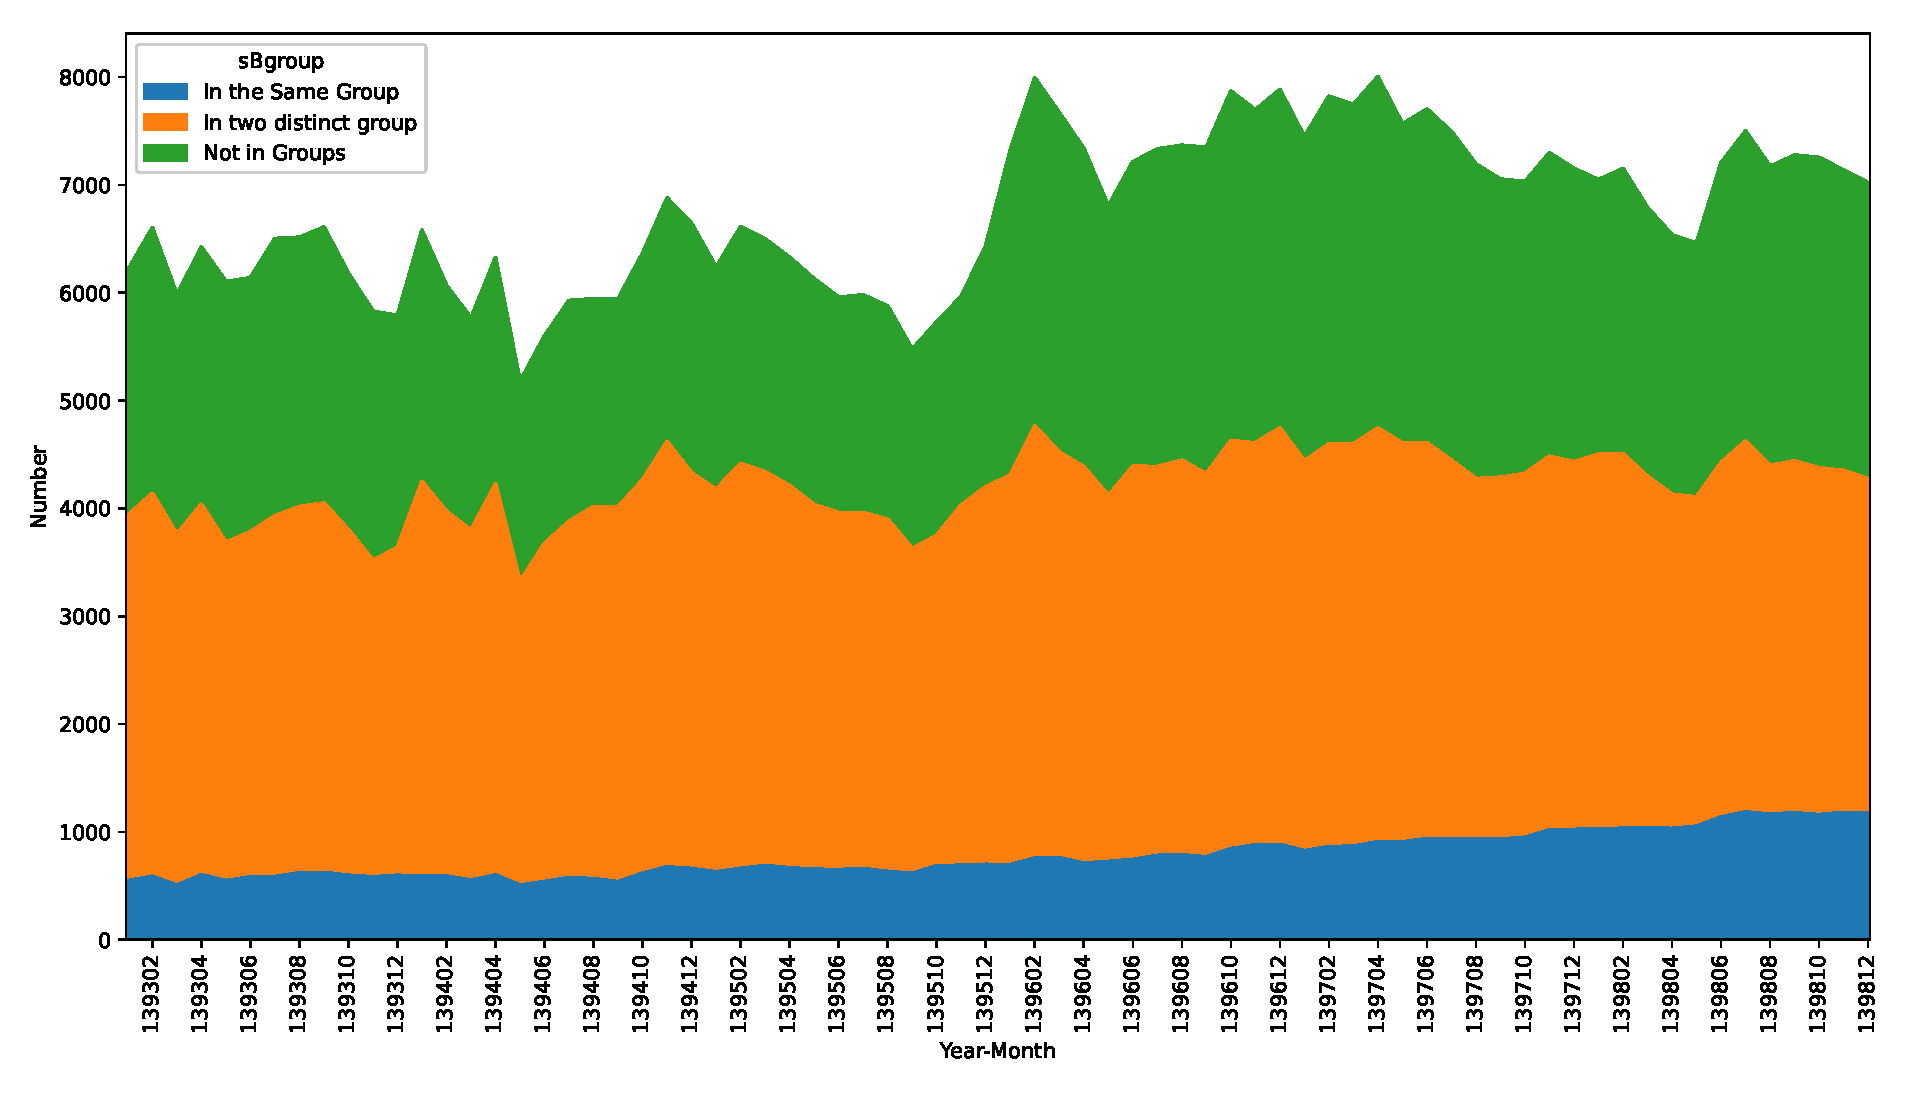
\includegraphics[width=\linewidth]{Output/idMonth.eps}
%\end{figure}
 
  \FloatBarrier
  
  
\subsection{\lr{Measurement of common-ownership}}

\begin{itemize}
	\item 
	جدول 
	\ref{maasurmentsSummary}
	خلاصه ملاک های استفاده شده در ادبیات
	\item 
	دو دسته ملاک اندازه گیری مالکیت مشترک
	\begin{itemize}
		\item 
		دارای پشتوانه مدل
		\begin{itemize}
			\item 
			توضیح تئوری دارند
			\item 
			تفسیر اقتصادی بهتری دارند
			\item 
			جهت دار
			\item
			در سطح صنعت یا شرکت
			\item
		\lr{	(e.g, \cite{harford2011institutional}; \cite{azar2018anticompetitive}; \cite{gilje2020s})}
		\end{itemize}
		\item 
	مدل های بدون پشتوانه
	\begin{itemize}
		\item 
		تفسیر اقتصادی مشخصی ندارند
		\item 
		شک است که چگونه انگیزخ مدیران را اندازه می گیرند
		\item 
		ویژگی های نامطلوبی دارند 
		\item
		محاسبه ساده است
		\item
		در سطح جفت و بدون جهت می توان محاسبه شود
		
		\item
		\lr{(e.g, \cite{AntonPolk}; \cite{azar2011new}; \cite{freeman2019effects}; \cite{hansen1996externalities};  \cite{he2017product}; \cite{he2019internalizing}; \cite{lewellen2021does}; \cite{newham2018common})}
	\end{itemize}
	
		
	\end{itemize}
	
	\item 
	هدف اصلی بررسی اثر مالکیت مشترک بر هم حرکتی در سطح جفت است
	
	\item 
	برای این هدف نیاز به ملاک در سطح جفت بدون جهت است با تفسیر اقتصادی مناسب
	
	\item 
	ملاک
	\cite{AntonPolk}
	میزان درصد مالکیت مشترک از مارکت دو شرکت است
	
	
	\item 
	از این ملاک استفاده می کنیم ولی مشکلی دارد
	\item 
	این ملاک توزیع مالکیت را در نظر نمی گیرد
		\item 
		برای همین از این ملاک استفاده می کنیم
		\begin{equation}
			\text{Overlap}_{Sqrt}(i, j) =  [\frac{\sum_{f =1}^{F}(\sqrt{S^f_{i,t}P_{i,t}}+\sqrt{S^f_{j,t}P_{j,t}})}{\sqrt{S_{i,t}P{i,t}} + \sqrt{S_{j,t}P{j,t}}}]^2 
			\label{sqrt0}
		\end{equation}
		\item
		در بخش 
		\ref{ModifiedMeasure}
		دلیل انتخاب این ملاک بیان شده است
\end{itemize}

\begin{LTR}
	\lr{\begin{table}[htbp]
	\centering
	\scriptsize
	\caption{ This table summarizes common ownership measurements in the literature.}
	\label{maasurmentsSummary}
	\resizebox{\textwidth}{!}{
		\begin{tabular}{cllc}
	\hline\hline
	\multicolumn{1}{c}{Group}      & \multicolumn{1}{c}{Paper} & \multicolumn{1}{c}{measurment} & \multicolumn{1}{c}{Flaws} \\
	\hline\hline
	\addlinespace
	\multicolumn{1}{c}{\multirow{5}[2]{*}{Model Based}} &  \cite{harford2011institutional}     &  \scriptsize  $
	\sum_{i\in I^{A,B}}\frac{\alpha_{i,B}}{\alpha_{i,A} + \alpha_{i,B}}     $     & Bi-directional \\
	\addlinespace 
	&  \cite{azar2018anticompetitive}     &  $   \sum_{j} \sum_k s_j s_k \frac{\sum_i \mu_{ij} \nu_{ik}}{\sum_i \mu_{ij} \nu_{ij}}   $     & Industry level \\
	\addlinespace
	&  \cite{gilje2020s}     &    $ \sum_{i = 1}^{I} \alpha_{i,A}g(\beta_{i,A})\alpha_{i,B}    $   & Bi-directional  \\
	\midrule
	\addlinespace 
	\multicolumn{1}{c}{\multirow{7}[5]{*}{Ad hoc}} & \cite{he2017product};      &  \multirow{2}{*}{$ \sum_{i\in I^{A,B}} 1 $}     & invariant to the level   \\
	& \cite{he2019internalizing} & & of ‌common ownership \\
	\addlinespace
	&  \cite{newham2018common}     &   $ \sum_{i\in I^{A,B}} min\{\alpha_{i,A},\alpha_{i,B}\} $    & ? \\
	\addlinespace
	& \multirow{2}{*}{   \cite{AntonPolk} }  &  \multirow{2}{*}{ $ \sum_{i\in I^{A,B}} \alpha_{i,A}\frac{\bar{\nu}_A}{\bar{\nu}_A +\bar{\nu}_B } + \alpha_{i,B}\frac{\bar{\nu}_B}{\bar{\nu}_A +\bar{\nu}_B }  $ }   &  Invariant to the  \\
	& & & decomposition of ownership \\
	\addlinespace
	& \cite{freeman2019effects}; & \multirow{2}{*}{ $ \sum_{i\in I^{A,B}} \alpha_{i,A} \times \sum_{i\in I^{A,B}} \alpha_{i,B} $ }&?\\
	&  \cite{hansen1996externalities} & & ?\\
	\hline\hline
\end{tabular}
	}
\end{table}
}

\end{LTR}




\begin{itemize}
	\item 
	در هر روز مالکیت مشترک با ملاک اصلاح شده تولید شده است
	\item 
مقدار میانگین ماهانه آن به عنوان مقدار ماهانه استفاده شده است
	\item 
جدول 
\ref{measureResults}
نتایج محاسبات برای مالکیت مشترک ملاک ساده 
(FCAP)
و اصلاح شده
(MFCAP)

\item
مالکیت مشترک برای گروه های کسب و کار حدودا 5 برابر و برای صنعت یکسان حدودا 3 برابر است

\begin{table}[htbp]
%	\centering
	\caption{ text}
	\label{measureResults}
	\resizebox{\textwidth}{!}
	{
		\begin{LTR}
			\lr{\begin{tabular}{lrrrrrrrrrr}
\toprule
\multirow{2}{*}{Subset}& \multicolumn{5}{c}{MFCAP} & \multicolumn{5}{c}{FCAP} \\
\cmidrule(lr){2-6} \cmidrule(lr){7-11}
&       mean &    std &    min & median &    max &         mean &    std &    min & median &    max \\
\midrule
All               &  0.15 &  0.24 &  0.00 &   0.06 &  4.62 &  0.12 &  0.16 &  0.0 &   0.05 &  0.97 \\
Same Group        &  0.47 &  0.41 &  0.00 &   0.41 &  4.04 &  0.38 &  0.25 &  0.0 &   0.37 &  0.97 \\
Not Same Group    &  0.10 &  0.16 &  0.00 &   0.04 &  2.90 &  0.08 &  0.11 &  0.0 &   0.04 &  0.97 \\
Same Industry     &  0.34 &  0.41 &  0.01 &   0.18 &  4.04 &  0.25 &  0.24 &  0.0 &   0.16 &  0.96 \\
Not Same Industry &  0.12 &  0.19 &  0.00 &   0.05 &  4.62 &  0.10 &  0.14 &  0.0 &   0.05 &  0.97 \\
\bottomrule
\end{tabular}
}
			\end{LTR}
	}
\end{table}


\end{itemize}

  \FloatBarrier
\subsection{\lr{Stock Return comovement}}
\label{comovement}
\begin{itemize}
	\item
	هم حرکتی ماهانه شرکت ها را محاسبه کرده ایم
	\item
	برای محاسبه هم حرکتی از باقی مانده مدل های فاکتوری استفاده کرده ایم
	\item
	با توجه به ویژگی بازار ایران شاخص صنعت را هم به مدل های چند فاکتوری اضافه کرده ایم

\begin{itemize}
	\item 
		\begin{equation}
		\begin{split}
			R_{i,t} =\alpha _{i}&+\beta _{mkt,i}{\mathit {R}}_{M,t} + \beta_{Ind,i}{\mathit {R}}_{Ind,t}+\beta _{HML,i}{\mathit {HML}}_{t} \\
			&+\beta _{SMB,i}{\mathit {SMB}}_{t}+\beta _{UMD,i}{\mathit {UMD}}_{t}+ \varepsilon_{i,t}
		\end{split}
		\label{e5Factor}
	\end{equation}
	\item
	از فاکتور های  [
	\lr{\cite{Carhart4Factor}}
	]
\end{itemize}
	
	\item
	برای محاسبه باقی مانده مدل ها، مدل را برای سه ماه ( از دو ماه قبل) پیش بینی می کنیم و بعد از آن باقی مانده ها را محاسبه می کنیم
	\item
	برای ماه مورد نظر هم بستگی باقی مانده ها را محاسبه می کنیم
	\item
	نتایج برای مدل های مختلف  در جدول
	\ref{tCorr}
	نشان داده شده است
	\item
	از مدل چهار عاملی به علاوه صنعت استفاده کرده ایم
	\begin{itemize}
		\item 
		با توجه به دامنه نوسان از تاخیر های فاکتور ها هم استفاده کردیم ولی نتایج  هم بستگی محاسبه شده تفاوت چندانی با مدل های قبلی نداشت
	\end{itemize}
	
\end{itemize}

     
\begin{LTR}
	\lr{ \begin{table}[htbp]
        \centering
        \caption{\footnotesize This table reports distribution of calculated correlation base on different models.}
        \label{tCorr}
        \resizebox{0.85\textwidth}{!}
        {
        \begin{tabular}{lrrrrr}
\toprule
{} &   mean &    std &  min &  median &  max \\
\midrule
 CAPM + Industry    &  0.018 &  0.205 & -1.0 &   0.018 &  1.0 \\
4 Factor            &  0.031 &  0.206 & -1.0 &   0.027 &  1.0 \\
4 Factor + Industry &  0.014 &  0.204 & -1.0 &   0.012 &  1.0 \\
\bottomrule
\end{tabular}

         }
      \end{table}}
\end{LTR}
      

\FloatBarrier


\subsection{Controls}

\begin{itemize}
	\item 
	هم حرکتی ممکن است ویژگی های شرکت ها ناشی شده باشد
	
	\item 
	اولین دسته کنترل ها برای جفت هاست
	\begin{itemize}
\item 
\textbf{SameIndustry} :
صنعت دو شرکت یکسان باشد
\item 
\textbf{SameGroup}:
دو شرکت در یک گروه کسب و کار قرار بگیرند
\item 
\textbf{CrossOwnership}:
حداکثر درصد مالکیت ضربدری میان دو شرکت
		
	\end{itemize}
	\item 
	جدول
	\ref{SameGroupIndustry}
	نشان داده است $5.7 \%$ از جفت های در یک صنعت
	$6.5 \%$ در یک گروه کسب و کار
	1\% نیز هم در یک گروه و هم در یک صنعت قرار دارد
	\item 
دسته دوم کنترل ها مشخصات شرکت ها را کنترل می کند
\begin{itemize}
	\item \textbf{Size1}:
	نرمالایزد رنک ترنسفرد اندازه شرکت بزرگتر
	
	
	\item \textbf{Size2}:
	نرمالایزد رنک ترنسفرد اندازه شرکت کوچکتر
	
	\item \textbf{BookToMarket1}:
	نرمالایزد رنک ترنسفرد نسبت بوک تو مارکت شرکت بزرگتر
	
	\item \textbf{BookToMarket2}:
		نرمالایزد رنک ترنسفرد نسبت بوک تو مارکت شرکت کوچکتر
	\item \textbf{SameSize}:
	منفی مقدار اختلاف اندازه رتبه صدکی دو شرکت نسبت به اندازه
	\item  \textbf{SameBookToMarket}:
	منفی مقدار اختلاف اندازه رتبه صدکی دو شرکت نسبت به بوک تو مارکت
\end{itemize}
	\item 
	متغیر ها مانند مقاله
	\lr{\cite{AntonPolk}}
	تعریف شده است
	\item
کنترل ها به صورت روزانه محاسبه شده اند و پس از آن میانگین ماهانه استفاده شده است
\item 
جدول 
\ref{ControlsSummary}
خلاصه آماری کنترل ها
\end{itemize}



\begin{LTR}
	\lr{\begin{table}[htbp]
\caption{\scriptsize This table reports the number of pairs in the same industry and business group.}
\label{SameGroupIndustry}
               \centering \scriptsize
         {

    \begin{tabular}{lcc}\hline\hline
    {Type of Pairs} & {Yes} &{No} \\
    \hline
    \addlinespace
    {SameIndustry} & 1760  & 16739 \\
          & \tiny(10\%) & \tiny (90\%) \\
          \addlinespace
{SameGroup} & 1118  & 17381 \\
          & \tiny(6\%) & \tiny (94\%) \\
          \addlinespace
{SameGroup \& SameIndustry} & 492  & 18007 \\
          & \tiny(3\%) & \tiny (97\%) \\    
                
          \hline\hline
    \end{tabular}%
                 }
             \end{table}}
\end{LTR}

\begin{LTR}
	\lr{ \begin{table}[htbp]
 \caption{\scriptsize This table shows the summary statistics of specified controls in empirical studies.}
 \label{ControlsSummary}
               \centering 
               \scriptsize
                \resizebox{\textwidth}{!}  {
    \begin{tabular}{lrrrrrrr}\hline\hline
          & \multicolumn{1}{l}{mean} & \multicolumn{1}{l}{std} & \multicolumn{1}{l}{min} & 25\%  & 50\%  & 75\%  & \multicolumn{1}{l}{max} \\
          \hline
          
          SameIndustry & 0.10  & 0.29  & 0.00  & 0.00  & 0.00  & 0.00  & 1.00 \\
          SameGroup & 0.06  & 0.23  & 0.00  & 0.00  & 0.00  & 0.00  & 1.00 \\
          Size1 & 0.72  & 0.21  & 0.01  & 0.58  & 0.78  & 0.91  & 1.00 \\
          Size2 & 0.43  & 0.25  & 0.00  & 0.23  & 0.42  & 0.62  & 0.99 \\
          SameSize & -0.29 & 0.21  & -0.97 & -0.42 & -0.24 & -0.12 & 0.00 \\
          BookToMarket1 & 0.53  & 0.26  & 0.00  & 0.34  & 0.54  & 0.73  & 1.00 \\
          BookToMarket2 & 0.52  & 0.24  & 0.00  & 0.34  & 0.52  & 0.71  & 1.00 \\
          SameBookToMarket & -0.30 & 0.19  & -0.99 & -0.42 & -0.26 & -0.15 & 0.00 \\
          MonthlyCrossOwnership & 0.01  & 0.05  & 0.00  & 0.00  & 0.00  & 0.00  & 0.96 \\
          
    
    \hline\hline
            \end{tabular}
                 }
             \end{table}}
\end{LTR}
         
         
 


\FloatBarrier


\section{Empirical Analysis}



\subsection{\lr{Forecasting Co-movement}}
\label{Forecasting Co-movement}

\begin{itemize}
	\item 
	در مرحله اول بررسی رابطه مالکیت مشترک و گروه های کسب و کار با هم حرکتی شرکت ها بررسی کرده ایم
	\item 
	در شکل 
	\ref{mcorr50}
	رابطه هم حرکتی دوره آینده با مالکیت مشترک در این دوره قابل مشاهده است
	 \begin{figure}[htbp]
		\centering  
		\centering
		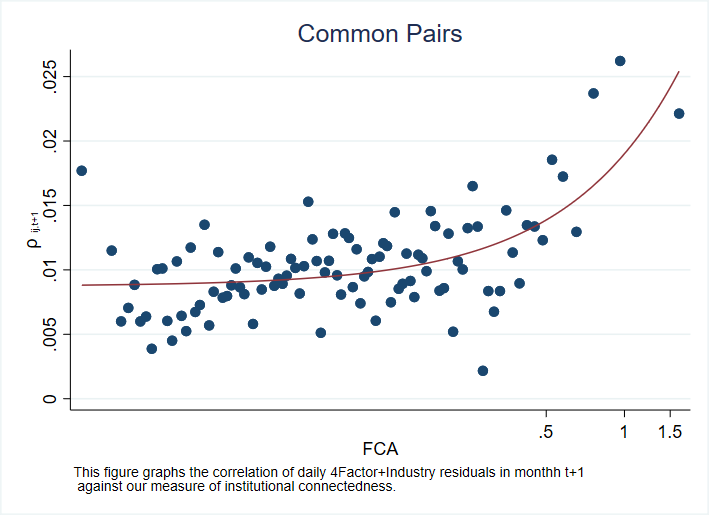
\includegraphics[width=0.7\linewidth]{"Output/mcorr50.eps"} 
		\caption{Future monthly correlation for different level of common ownership at this period }
		\label{mcorr50}
	\end{figure}
	\item 
	هم حرکتی دوره آینده را بر روی متغیر های مورد نظر برآورد می کنیم:
	\begin{equation}
\begin{split}
\rho_{ij,t+1} = & \text{ 	}\beta_0 + \beta_1* \text{FCA}^*_{ij,t} + \beta_2* \text{SameGroup}_{ij} \\
 &	+\beta_3* \text{FCA}^*_{ij,t} \times \text{SameGroup}_{ij}   \\
  & + \sum_{k=1} ^{n} \alpha_k*\text{Control}_{ij,t} + \varepsilon_{ij,t+1}
\end{split}
\label{model1}
\end{equation}
	
	\item
	برای هر ماه این معادله برآورد می شود و متوسط سری زمانی ضرایب به شیوه
	
	\lr{\cite{FamaMacBeth}}
	برآورد شده است
	\item
	این شیوه انتخاب شده است تا مشکلی با 
	\lr{cross-correlation}
	نداشته باشیم
	\item
	انحراف معیار هم به شیوه
	
	\lr{\cite{newey1987hypothesis}}
	اصلاح شده است تا 
	\lr{autocorrelation}
	را بر طرف کنید
	\item
	تا 4 دوره قبل را بر طرف می کنید
	($ 4(71/100)^{\frac{2}{9}} = 3.71 \sim 4 $)
	
	
\end{itemize}

\begin{itemize}
	\item 
	نتایج برآورد در جدول 
	\ref{mresult2part1}
	و
	\ref{mresult2part2}
	نشان داده شده است
	
\begin{itemize}
\item
جدول
\ref{mresult2part1}
\begin{itemize}

	\item 
	در دو ستون اول  اثر مالکیت مشترک بر روی هم حرکتی بررسی کرده ایم
	\item 
		در ستون 3 و 4 فقط گروه های کسب و کار را براورد کرده ایم حدودا $1.5$ درصد هم حرکتی افزایش پیدا می کند
	\item 
	اثر گروه کسب و کار بیشتر از مالکیت مشترک است
	\item 
	با اضافه کردن گروه کسب و کار و مالکیت مشترک، مالکیت مشترک اثر خود را از دست می دهد
\end{itemize}
	
\item
جدول
\ref{mresult2part2}
\begin{itemize}
	\item 
	مالکیت مشترک فقط در گروه های کسب و کار اثر دارد
	\item
	در دو ستون اخر هم بدون محدود کردن جامعه بودن در گروه را بررسی کرده ایم و یافتیم که در گروه کسب و کار مالکیت مشترک اهمیت دارد
	\item
	ستون آخر اثر ثابت گروه های کسب و کار را اضافه کردیم نتایج برقرار است
\end{itemize}
	
\end{itemize} 
\end{itemize}

	{\begin{table}[p]
	\centering
	\caption{Connected Co-movement}
	\label{mresult2part1}
	\resizebox{1\textwidth}{!}{
		\begin{LTR}
			\lr{{
\def\sym#1{\ifmmode^{#1}\else\(^{#1}\)\fi}
\begin{tabular}{l*{6}{c}}
\hline\hline
                    &\multicolumn{6}{c}{Dependent Variable:  Future Pairs's Comovement}                                                                 \\\cmidrule(lr){2-7}
                    &\multicolumn{1}{c}{(1)}         &\multicolumn{1}{c}{(2)}         &\multicolumn{1}{c}{(3)}         &\multicolumn{1}{c}{(4)}         &\multicolumn{1}{c}{(5)}         &\multicolumn{1}{c}{(6)}         \\
\hline
$ \text{MFCAP*} $   &     0.00600\sym{***}&     0.00328\sym{***}&                     &                     &     0.00104         &    0.000929         \\
                    &      (8.10)         &      (4.87)         &                     &                     &      (1.68)         &      (1.53)         \\
[1em]
SameGroup           &                     &                     &      0.0358\sym{***}&      0.0254\sym{***}&      0.0242\sym{***}&      0.0219\sym{***}\\
                    &                     &                     &      (9.99)         &      (8.45)         &      (8.21)         &      (7.02)         \\
[1em]
SameIndustry        &                     &      0.0267\sym{***}&                     &      0.0216\sym{***}&      0.0212\sym{***}&      0.0215\sym{***}\\
                    &                     &      (7.39)         &                     &      (6.81)         &      (6.72)         &      (6.80)         \\
[1em]
SameBM              &                     &      0.0224\sym{***}&                     &      0.0213\sym{***}&      0.0214\sym{***}&      0.0199\sym{***}\\
                    &                     &      (6.41)         &                     &      (6.09)         &      (6.16)         &      (5.77)         \\
[1em]
SameSize            &                     &      0.0123\sym{**} &                     &      0.0143\sym{***}&      0.0138\sym{***}&      0.0254\sym{***}\\
                    &                     &      (3.24)         &                     &      (3.85)         &      (3.71)         &      (5.56)         \\
[1em]
CrossOwnership      &                     &      0.0600\sym{***}&                     &      0.0300\sym{*}  &      0.0316\sym{*}  &      0.0377\sym{**} \\
                    &                     &      (5.50)         &                     &      (2.36)         &      (2.48)         &      (2.93)         \\
[1em]
Constant            &      0.0142\sym{***}&      0.0204\sym{***}&      0.0103\sym{***}&      0.0187\sym{***}&      0.0188\sym{***}&      0.0280\sym{***}\\
                    &     (12.80)         &      (8.91)         &      (9.42)         &      (7.99)         &      (8.04)         &      (9.43)         \\
\hline
PairType Control    &          No         &          No         &          No         &          No         &          No         &         Yes         \\
Observations        &      389591         &      389591         &      389591         &      389591         &      389591         &      389591         \\
\hline\hline  \end{tabular}}
}
		\end{LTR}
	}
\end{table}}

	{\begin{table}[p]
	\centering
	\caption{Connected Co-movement}
	\label{mresult2part2}
	\resizebox{1\textwidth}{!}{
		\begin{LTR}
			\lr{{
\def\sym#1{\ifmmode^{#1}\else\(^{#1}\)\fi}
\begin{tabular}{l*{4}{c}}
\hline\hline
                &\multicolumn{4}{c}{Dependent Variable: Future Pairs's co-movement'}        \\\cmidrule(lr){2-5}
                &\multicolumn{1}{c}{(1)}         &\multicolumn{1}{c}{(2)}         &\multicolumn{1}{c}{(3)}         &\multicolumn{1}{c}{(4)}         \\
\hline
$ \text{MFCAP*} $&  0.00944\sym{***}& 0.000397         & 0.000377         &-0.0000113         \\
                &   (7.24)         &   (0.68)         &   (0.65)         &  (-0.02)         \\
[1em]
Same Group      &                  &                  &  0.00624\sym{**} &  0.00549\sym{*}  \\
                &                  &                  &   (2.81)         &   (2.27)         \\
[1em]
 $ (\text{MFCAP}^*) \times {\text{SameGroup} }  $ &                  &                  &  0.00992\sym{***}&   0.0107\sym{***}\\
                &                  &                  &   (6.49)         &   (6.97)         \\
\hline
Observations    &    58337         &  1607659         &  1665996         &  1665996         \\
Sub-sample      &SameGroup         &   Others         &      All         &      All         \\
Group Effect    &       No         &       No         &       No         &      Yes         \\
Controls        &      Yes         &      Yes         &      Yes         &      Yes         \\
$ R^2 $         &   0.0112         & 0.000577         & 0.000898         &  0.00575         \\
\hline\hline
\multicolumn{5}{l}{\footnotesize \textit{t} statistics in parentheses}\\
\multicolumn{5}{l}{\footnotesize \sym{*} \(p<0.05\), \sym{**} \(p<0.01\), \sym{***} \(p<0.001\)}\\
\end{tabular}
}
}
		\end{LTR}
	}
\end{table}}


% \begin{landscape}
%
%	{\begin{table}[p]
%	\centering
%	\caption{Connected Co-movement}
%	\label{mresult2}
%	\resizebox{1.2\textwidth}{!}{
%		\begin{LTR}
%			\lr{{
\def\sym#1{\ifmmode^{#1}\else\(^{#1}\)\fi}
\begin{tabular}{l*{7}{c}}
\hline\hline
                &\multicolumn{7}{c}{Dependent Variable: Future Monthly Correlation of 4F+Industry Residuals}                                         \\\cmidrule(lr){2-8}
                &\multicolumn{1}{c}{(1)}         &\multicolumn{1}{c}{(2)}         &\multicolumn{1}{c}{(3)}         &\multicolumn{1}{c}{(4)}         &\multicolumn{1}{c}{(5)}         &\multicolumn{1}{c}{(6)}         &\multicolumn{1}{c}{(7)}         \\
\hline
Same Group      &   0.0138\sym{***}&   0.0128\sym{***}&                  &                  &  0.00978\sym{***}&  0.00458         &  0.00356         \\
                &   (5.76)         &   (6.29)         &                  &                  &   (4.29)         &   (1.43)         &   (1.11)         \\
[1em]
$ \text{FCA*} $ &                  &                  &  0.00405\sym{***}&  0.00375\sym{***}&  0.00296\sym{***}&  0.00258\sym{***}&  0.00273\sym{***}\\
                &                  &                  &   (4.94)         &   (5.12)         &   (3.77)         &   (3.53)         &   (3.51)         \\
[1em]
 $ (\text{FCA}^*) \times {\text{SameGroup} }  $ &                  &                  &                  &                  &                  &  0.00524\sym{**} &  0.00517\sym{**} \\
                &                  &                  &                  &                  &                  &   (3.21)         &   (3.18)         \\
\hline
Observations    &   388492         &   388492         &   388492         &   388492         &   388492         &   388492         &   388492         \\
Group Effect    &       No         &       No         &       No         &       No         &       No         &       No         &      Yes         \\
Controls        &       No         &      Yes         &       No         &      Yes         &      Yes         &      Yes         &      Yes         \\
$ R^2 $         & 0.000404         &  0.00200         & 0.000423         &  0.00201         &  0.00229         &  0.00245         &  0.00875         \\
\hline\hline
\multicolumn{8}{l}{\footnotesize \textit{t} statistics in parentheses}\\
\multicolumn{8}{l}{\footnotesize \sym{*} \(p<0.05\), \sym{**} \(p<0.01\), \sym{***} \(p<0.001\)}\\
\end{tabular}
}
}
%		\end{LTR}
%	}
%\end{table}}
% \end{landscape}
\FloatBarrier



\subsection{\lr{High level of common ownership}}
\begin{itemize}
	\item 
	با توجه به جدول 
	\ref{measureResults}
	گروه های کسب و کار به صورت مالکیت بالاتر نیز دارند 
	\item
	برای برطرف کردن این مسئله بررسی را محدود به مالکیت مشترک بالا کردیم
	\item
	با توجه به شکل 
	\ref{Qmcorr5subsample}
	بالاتر از کوارتر سوم داده به نظر می آید بیشترین تاثیر را در هم حرکتی دارد
	
	\begin{figure}[htbp]
		\centering  
		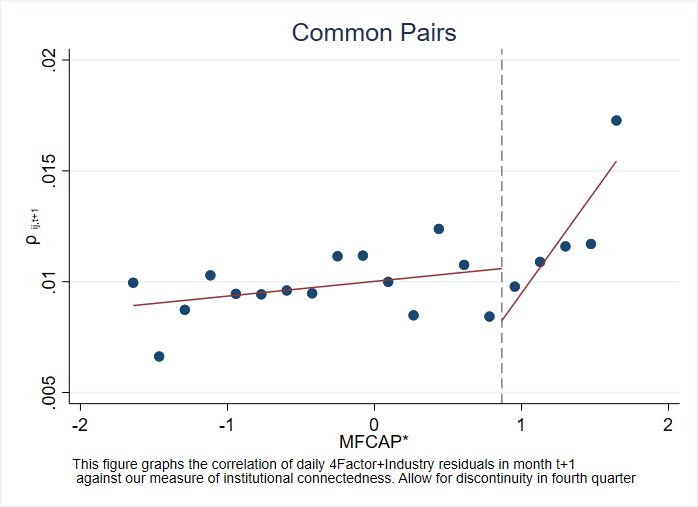
\includegraphics[width=0.6\linewidth]{"Output/Qmcorr5lrd.eps"}
		\caption{text}
		\label{Qmcorr5lrd}
	\end{figure}
	\begin{figure}[htbp]
		\centering  
		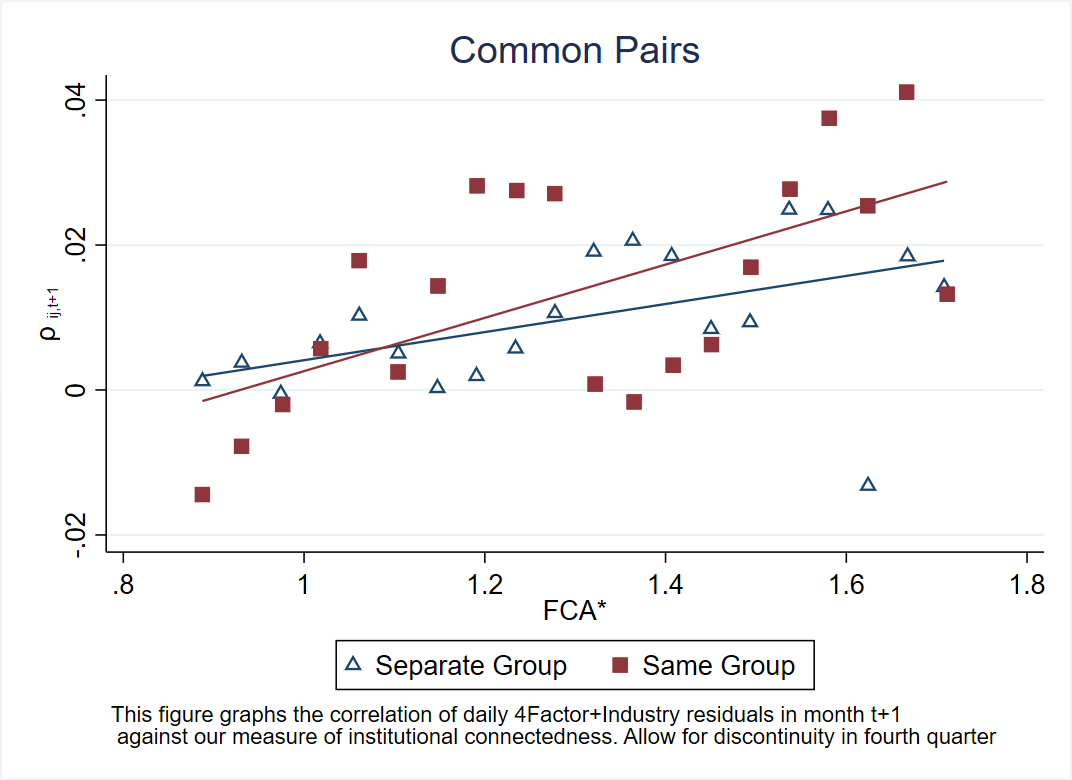
\includegraphics[width=0.45\linewidth]{"Output/Qmcorr5lrdbgsubsample.eps"}
		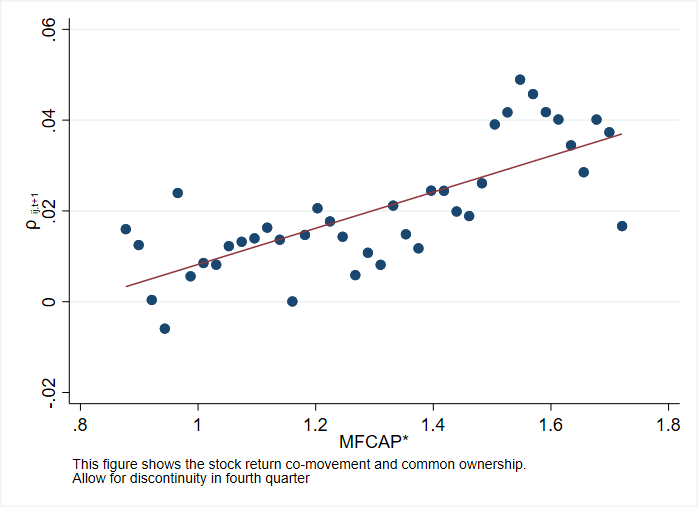
\includegraphics[width=0.45\linewidth]{"Output/Qmcorr5subsample.eps"}
		\caption{text}
		\label{Qmcorr5subsample}
	\end{figure}

	\item
	بررسی را محدود به جفت های دراای مالکیت زیاد کردیم و مدل 
	\ref{model1}
	را به شیوه گذشته برآورد کریدم
	\item
	نتایج در جدول 
	 \ref{QTimemresult2subsample}
	 نتایج را نشان داده است
\lr{\begin{LTR}
			 \begin{table}[htbp]
	 	\centering
	 	\caption{\scriptsize Estimation results for high level of common ownership}
	 	\label{QTimemresult2subsample}
	 	\resizebox{\textwidth}{!}{
	 		{
\def\sym#1{\ifmmode^{#1}\else\(^{#1}\)\fi}
\begin{tabular}{l*{7}{c}}
\hline\hline
                &\multicolumn{7}{c}{Dependent Variable:  Future Pairs's Comovement}                                                                  \\\cmidrule(lr){2-8}
                &\multicolumn{1}{c}{(1)}         &\multicolumn{1}{c}{(2)}         &\multicolumn{1}{c}{(3)}         &\multicolumn{1}{c}{(4)}         &\multicolumn{1}{c}{(5)}         &\multicolumn{1}{c}{(6)}         &\multicolumn{1}{c}{(7)}         \\
\hline
SameGroup       &   0.0254\sym{***}&                  &   0.0249\sym{***}&                  &                  &  0.00477         &  0.00252         \\
                &   (8.45)         &                  &   (8.21)         &                  &                  &   (1.32)         &   (0.66)         \\
[1em]
$ (\text{MFCAP} > \text{Larger than 75th Percentile}) $ &                  &  0.00660\sym{***}& 0.000777         &   0.0230\sym{***}& -0.00258\sym{*}  & -0.00157         &-0.000513         \\
                &                  &   (5.48)         &   (0.73)         &   (7.09)         &  (-2.00)         &  (-1.29)         &  (-0.46)         \\
[1em]
 $ (\text{MFCAP} > Q3[\text{MFCAP}]) \times {\text{SameGroup}} $ &                  &                  &                  &                  &                  &   0.0248\sym{***}&   0.0237\sym{***}\\
                &                  &                  &                  &                  &                  &   (7.24)         &   (7.34)         \\
\hline
Sub-sample      &      All         &      All         &      All         &SameGroup         &   Others         &      All         &      All         \\
Controls        &      Yes         &      Yes         &      Yes         &      Yes         &      Yes         &      Yes         &      Yes         \\
Business Group FE&       No         &       No         &       No         &       No         &       No         &       No         &      Yes         \\
Observations    &   389591         &   389591         &   389591         &    47076         &   342515         &   389591         &   389591         \\
\hline\hline
\multicolumn{8}{l}{\footnotesize \textit{t} statistics in parentheses}\\
\multicolumn{8}{l}{\footnotesize \sym{*} \(p<0.05\), \sym{**} \(p<0.01\), \sym{***} \(p<0.001\)}\\
\end{tabular}
}

	 	}
	 \end{table}
\end{LTR}}
	\begin{itemize}
		\item 
		همچنان نتایج گذشته تایید شده است
		\item 
	مالکیت مشترک صرفا در گروه های کسب و کار اهمیت دارد 
		\item 
		گروه های کسب و کار بیشترین تاثیر را در میان سطح زیاد مالیکت مشترک دارد
		\item 
		ممکن است جفت های دارای مالکیت بالا تفاوت بنیادی با دیگر جفت ها داشته باشند 
		\begin{itemize}
			\item 
			در شکل 
			\ref{QarterSummary}
			متوسط کنترل های تعریف شده نشان داده شده است
			\begin{figure}[htbp]
				\centering  
				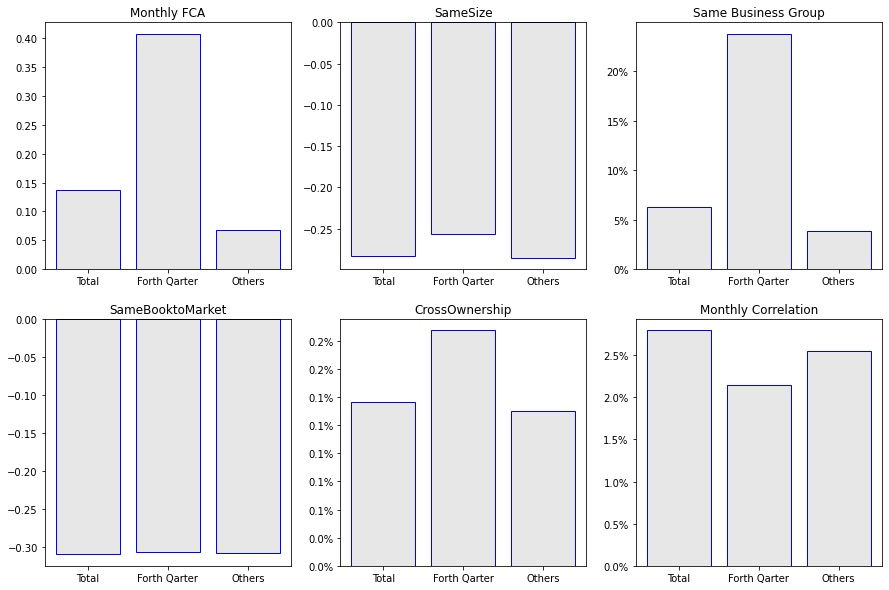
\includegraphics[width=0.85\linewidth]{"Output/QarterSummary.eps"}
				\caption{Pairs' characteristics for the pairs with high level of common ownership}
				\label{QarterSummary}
			\end{figure}
		\item
		تفاوت چشمگیری نسبت به بقیه جامعه ندارند
		\end{itemize}
	\end{itemize}
	
	
\end{itemize}


\FloatBarrier

\subsection{All Pairs}
\begin{itemize}
	\item 
	اگر گروه های کسب و کار اهمیت داشته باشند نیاز نیست تا محاسبات را محدود به شرکت های دارای مالک مشترک کنیم
	\item
	همه جفت های بازار را تشکیل می دهیم
	\item
	زمانی که مالکیت مشترک وجود ندارد مالکیت مشترک را برابر صفر قرار می دهیم و اگر مالکیت مشترک داشته باشند میزان ارن را محاسبه می کنیم
	\item
	برای همه جفت ها مدل 
	\ref{model1}
	را به شیوه گذشته برآورد می کنیم
	\item
	نتایج در جدول 
	\ref{AllPairs}
	نشان داده شده است
	\begin{itemize}
		\item 
		در ستون اول عضویت در گروه کسب و کار را نشان می دهد که علامت و مقدار برآورد قبلی را نشان می دهد
		\item 
		در ستون2 نیز برای سطح مالکیت مشترک بررسی شده است و نتایج قبلی تایید شده است
		\item 
		در میان گروه کسب و کار سطح مالکیت مشترک تاثیر چندانی ندارد
		\item
		درمیان جفت های بیرون گروه کسب و کار نیز سطح مالکیت مشترک اهمیت دارد که می تواند صرفا اهمیت مالکیت مشترک در پیش بینی هم حرکتی قیمت شرکت ها را نشان دهد.
			\begin{table}[htbp]
					%	\centering
					\caption{Non-connected Co-movement}
					\label{AllPairs}
					\resizebox{1\textwidth}{!}{
					\begin{LTR}
						\lr{	{
\def\sym#1{\ifmmode^{#1}\else\(^{#1}\)\fi}
\begin{tabular}{l*{7}{c}}
\hline\hline
                &\multicolumn{7}{c}{Dependent Variable: Future Pairs' co-movement}                                                                   \\\cmidrule(lr){2-8}
                &\multicolumn{1}{c}{(1)}         &\multicolumn{1}{c}{(2)}         &\multicolumn{1}{c}{(3)}         &\multicolumn{1}{c}{(4)}         &\multicolumn{1}{c}{(5)}         &\multicolumn{1}{c}{(6)}         &\multicolumn{1}{c}{(7)}         \\
\hline
SameGroup       &   0.0156\sym{***}&                  &   0.0158\sym{***}&                  &                  &   0.0138\sym{***}&   0.0131\sym{***}\\
                &   (9.84)         &                  &  (10.22)         &                  &                  &   (8.27)         &   (7.68)         \\
[1em]
$ \text{MFCAP*}  $&                  &-0.0000723         &-0.000277         &  0.00169         &-0.000322\sym{*}  &-0.000390\sym{**} &-0.000427\sym{*}  \\
                &                  &  (-0.44)         &  (-1.80)         &   (1.42)         &  (-2.19)         &  (-2.70)         &  (-2.29)         \\
[1em]
 $ (\text{MFCAP}^*) \times {\text{SameGroup} }  $ &                  &                  &                  &                  &                  &  0.00313\sym{**} &  0.00364\sym{**} \\
                &                  &                  &                  &                  &                  &   (2.80)         &   (3.34)         \\
\hline
Controls        &      Yes         &      Yes         &      Yes         &      Yes         &      Yes         &      Yes         &      Yes         \\
Sub-Sample      &    Total         &    Total         &    Total         &SameGroups         &   Others         &    Total         &    Total         \\
Business Group FE&       No         &       No         &       No         &       No         &       No         &       No         &      Yes         \\
Observations    &  6018646         &  6018646         &  6018646         &   114526         &  5904120         &  6018646         &  6018646         \\
\hline\hline
\multicolumn{8}{l}{\footnotesize \textit{t} statistics in parentheses}\\
\multicolumn{8}{l}{\footnotesize \sym{*} \(p<0.05\), \sym{**} \(p<0.01\), \sym{***} \(p<0.001\)}\\
\end{tabular}
}

					}
					\end{LTR}}
				\end{table}
	\end{itemize}
	
\end{itemize}






\FloatBarrier




%\subsection{\lr{Size effect}}
%\begin{itemize}
%	\item 
%	مقاله
%	\lr{\cite{AntonPolk}}
%	بررسی اصلی را محدود به شرکت های بزرگ کرده بود
%	\item 
%	بررسی می کنیم آیا اثر به اندازه شرکت ها وابسته است یا خیر
%	\item 
%	شرکت های بزرگتر از میانه ارزش بازار را شرکت های بزرگ دسته بندی می کنیم
%	\item 
%	سه نوع جفت تولید می شود جفت های بزرگ، ترکیبی و کوچک
%	\item 
%	که آنالیز 
%	\lr{\cite{AntonPolk}}
%	فقط برای جفت های بزرگ صورت گرفته است
%	\item 
%	شکل 
%	\ref{mcorrPairType}
%	نشان داده شده است
%	\begin{figure}[htbp]
%		\centering  
%		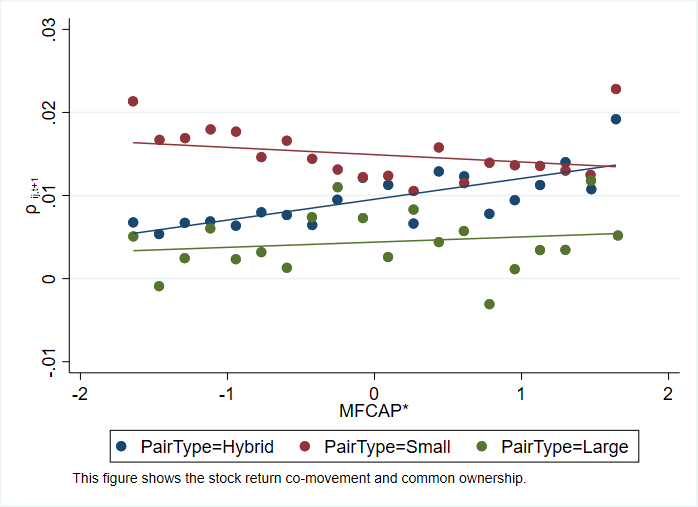
\includegraphics[width=0.7\linewidth]{"Output/mcorrPairType.eps"}
%		\caption{text}
%		\label{mcorrPairType}
%	\end{figure}
%	\item 
%	در ابتدا انالیز اصلی را برای جفت های دارای مالک مشترک انجام دادیم
%	\item
%	جدول  
%	\ref{Qmresult4}
%	نشان داده است
%		\begin{LTR}
%		\lr{\begin{table}[htbp]
%				\centering
%				\caption{text}
%				\label{Qmresult4}
%				\resizebox{1\textwidth}{!}{
%					{
\def\sym#1{\ifmmode^{#1}\else\(^{#1}\)\fi}
\begin{tabular}{l*{8}{c}}
\hline\hline
                &\multicolumn{8}{c}{Dependent Variable: Future Monthly Correlation of 4F+Ind. Res.}                                                                     \\\cmidrule(lr){2-9}
                &\multicolumn{1}{c}{(1)}         &\multicolumn{1}{c}{(2)}         &\multicolumn{1}{c}{(3)}         &\multicolumn{1}{c}{(4)}         &\multicolumn{1}{c}{(5)}         &\multicolumn{1}{c}{(6)}         &\multicolumn{1}{c}{(7)}         &\multicolumn{1}{c}{(8)}         \\
\hline
$ \text{FCA*} $ & 0.000377         & 0.000698         &-0.000175         &  0.00199\sym{***}&  0.00177\sym{**} & -0.00151         & -0.00177         &-0.0000771         \\
                &   (0.65)         &   (1.25)         &  (-0.31)         &   (3.56)         &   (3.00)         &  (-1.58)         &  (-1.84)         &  (-0.14)         \\
[1em]
Same Group      &  0.00624\sym{**} &   0.0102\sym{***}& -0.00153         &   0.0117\sym{***}&  0.00661\sym{*}  &   0.0366\sym{***}&   0.0268\sym{***}&  0.00750\sym{***}\\
                &   (2.81)         &   (3.95)         &  (-0.53)         &   (3.76)         &   (2.15)         &  (10.31)         &   (6.57)         &   (3.53)         \\
[1em]
 $ (\text{FCA}^*) \times {\text{SameGroup} }  $ &  0.00992\sym{***}&                  &   0.0134\sym{***}&                  &  0.00599\sym{*}  &                  &   0.0123\sym{***}&   0.0105\sym{***}\\
                &   (6.49)         &                  &   (4.80)         &                  &   (2.34)         &                  &   (4.17)         &   (6.72)         \\
\hline
Observations    &  1665996         &   346170         &   346170         &   693728         &   693728         &   626098         &   626098         &  1665996         \\
Controls        &      Yes         &      Yes         &      Yes         &      Yes         &      Yes         &      Yes         &      Yes         &      Yes         \\
Sub-sample      &All Firms         &Big Firms         &Big Firms         &Big \& Small Firms         &Big \& Small Firms         &Small Firms         &Small Firms         &All Firms         \\
Pair Size FE    &       No         &       No         &       No         &       No         &       No         &       No         &       No         &      Yes         \\
$ R^2 $         & 0.000898         &  0.00193         &  0.00232         &  0.00135         &  0.00149         &  0.00180         &  0.00198         &  0.00130         \\
\hline\hline
\multicolumn{9}{l}{\footnotesize \textit{t} statistics in parentheses}\\
\multicolumn{9}{l}{\footnotesize \sym{*} \(p<0.05\), \sym{**} \(p<0.01\), \sym{***} \(p<0.001\)}\\
\end{tabular}
}

%				}
%		\end{table}}
%	\end{LTR}
%	\begin{itemize}
%		\item 
%		در جفت های بزرگ و کوچک نتایج با نتایج اولیه همسان است
%		\item 
%		در حفت های ترکیبی همچنان مالکیت مشترک و عضویت در گروه کسب و کار اهمیت دارد
%		
%	\end{itemize}
%	\item
%	سپس انالیز را برای تمام  جفت های بازار  انجام دادیم
%	\item
%	جدول  
%	\ref{Qmresult4AllPairs}
%	نشان داده است
%	\begin{LTR}
%		\lr{	\begin{table}[htbp]
%				\centering
%				\caption{text}
%				\label{Qmresult4AllPairs}
%				\resizebox{1\textwidth}{!}{
%					{
\def\sym#1{\ifmmode^{#1}\else\(^{#1}\)\fi}
\begin{tabular}{l*{8}{c}}
\hline\hline
                &\multicolumn{8}{c}{Dependent Variable: Future Monthly Correlation of 4F+Ind. Res.}                                                                     \\\cmidrule(lr){2-9}
                &\multicolumn{1}{c}{(1)}         &\multicolumn{1}{c}{(2)}         &\multicolumn{1}{c}{(3)}         &\multicolumn{1}{c}{(4)}         &\multicolumn{1}{c}{(5)}         &\multicolumn{1}{c}{(6)}         &\multicolumn{1}{c}{(7)}         &\multicolumn{1}{c}{(8)}         \\
\hline
SameGroup       &   0.0134\sym{***}&  0.00954\sym{***}&  0.00853\sym{***}&   0.0136\sym{***}&   0.0118\sym{***}&   0.0314\sym{***}&   0.0267\sym{***}&   0.0138\sym{***}\\
                &   (7.81)         &   (4.63)         &   (3.71)         &   (7.35)         &   (6.46)         &  (10.19)         &   (7.93)         &   (8.27)         \\
[1em]
$ \text{FCA*} $ & 0.000408\sym{*}  &-0.0000120         &-0.000115         & 0.000514\sym{*}  & 0.000401         & -0.00143\sym{***}& -0.00154\sym{***}&-0.000390\sym{**} \\
                &   (2.11)         &  (-0.05)         &  (-0.47)         &   (2.09)         &   (1.67)         &  (-3.86)         &  (-3.97)         &  (-2.70)         \\
[1em]
 $ (\text{FCA}^*) \times {\text{SameGroup} }  $ &  0.00247\sym{*}  &                  &  0.00178         &                  &  0.00272         &                  &  0.00545\sym{**} &  0.00313\sym{**} \\
                &   (2.15)         &                  &   (1.30)         &                  &   (1.59)         &                  &   (3.38)         &   (2.80)         \\
\hline
Observations    &  6018646         &  1753614         &  1753614         &  2992221         &  2992221         &  1272811         &  1272811         &  6018646         \\
Controls        &      Yes         &      Yes         &      Yes         &      Yes         &      Yes         &      Yes         &      Yes         &      Yes         \\
Sub-sample      &All Firms         &Large Firms         &Large Firms         &Hybrid Firms         &Hybrid Firms         &Small Firms         &Small Firms         &All Firms         \\
Pair Size FE    &       No         &       No         &       No         &       No         &       No         &       No         &       No         &      Yes         \\
$ R^2 $         & 0.000515         & 0.000796         & 0.000860         & 0.000688         & 0.000735         &  0.00191         &  0.00199         & 0.000829         \\
\hline\hline
\multicolumn{9}{l}{\footnotesize \textit{t} statistics in parentheses}\\
\multicolumn{9}{l}{\footnotesize \sym{*} \(p<0.05\), \sym{**} \(p<0.01\), \sym{***} \(p<0.001\)}\\
\end{tabular}
}

%				}
%		\end{table}}
%	\end{LTR}
%	\begin{itemize}
%	\item 
%	برای جفت های بزرگ صرفا گروه های کسب و کار اهمیت دارد 
%	\item 
%	برای جفت های بزرگ اصلا مالکیت مشترک اهمیت ندارد
%	\item 
%	در جفت های کوجک گروه کسب و کار اثر مثبت و مالکیت مشترک بیرون گروه کسب و کار اثر منفی دارد 
%	\item
%	در جفت های ترکیبی نیز مالکیت مشترک اثر کمتری از گروه کسب و کار دارد
%	
%\end{itemize}
%\end{itemize}
%		
%
%
%	
	





\FloatBarrier


%\section{\lr{Evidence for correlated trading} }
\begin{itemize}
	\item 
	به نظر می آید در شرکت های عضو گروه های کسب و کار به همراه یکدیگر معامله می شوند
	\item
	از ملاک های اندازه گیری معاملات برای این هدف استفاده کرده یم
\end{itemize}
\subsection{\lr{Turnover}}
\begin{itemize}
	\item 
	از تغییرات 
	\lr{turnover}
	برای بررسی معامله هم زمان استفاده می کنیم
	\item 
	تعریف تغییرات انحراف معیار
	\begin{equation}
			\Delta \text{TurnOver} = \ln(\frac{\text{TurnOver}_{i,t}}{\text{TurnOver}_{i,t-1}}) = 
		\ln({\frac{\text{volume}_{i,t}}{\text{MarketCap}_{i,t}}}) - \ln({\frac{\text{volume}_{i,t-1}}{\text{MarketCap}_{i,t-1}}})
	\end{equation}
	\item 
	از شیوه مقاله 
	\lr{\cite{Liquidity2016}}
	برای تعریف استفاده کرده ایم
\end{itemize}


\begin{itemize}
	\item
	به منظور بررسی معامله هم زمان شرکت ها در گروه نیاز است تا رابطه تغییرات 
	\lr{turnover}
	را با میانگین تغییرات 
	\lr{turnover}
	در گروه بدست بیاوریم
	\item 
	مدل زیر را برآورد می کنیم
	\begin{equation*}
	\begin{split}
		\Delta \text{Turnover}_{i,t} =  & \text{	}\alpha + \beta_{Market,t} \Delta \text{Turnover}_{Market,t}  
		+ \beta_{Ind,t} \Delta \text{Turnover}_{Ind,t} \\ & + \beta_{Group,t} \Delta \text{Turnover}_{Group,t} + \delta\text{Controls} + \varepsilon_{i,t}
	\end{split}
\end{equation*}
	\item
	انتظار داریم متوسط ضرایب برای تغییرات
	\lr{turnover}
	گروه معنا دار و مثبت باشد
	\item
	جدول 
	\ref{turnover}
	نتایج برآورد را نشان می دهد
	\begin{LTR}
		\lr{\begin{table}[htbp]
				\centering
				\caption{cross-sectional average of the time-series coefficients for daily changes in turnover }
				\resizebox{1\textwidth}{!}{
					{
\def\sym#1{\ifmmode^{#1}\else\(^{#1}\)\fi}
\begin{tabular}{l*{4}{c}}
\hline\hline
                    &\multicolumn{4}{c}{Dependent Variable: $\Delta \text{TurnOver}\_{i} $ }                 \\\cmidrule(lr){2-5}
                    &\multicolumn{1}{c}{(1)}         &\multicolumn{1}{c}{(2)}         &\multicolumn{1}{c}{(3)}         &\multicolumn{1}{c}{(4)}         \\
\hline
 $ \Delta \text{TurnOver}_{\text{Market}} $ &       0.416\sym{***}&       0.326\sym{***}&       0.252\sym{***}&       0.228\sym{***}\\
                    &     (12.25)         &      (5.35)         &      (6.41)         &      (4.24)         \\
[1em]
 $ \Delta \text{TurnOver}_{\text{Industry-i}} $ &       0.142\sym{***}&       0.213\sym{***}&      0.0335         &       0.167\sym{**} \\
                    &      (3.79)         &      (6.29)         &      (1.34)         &      (2.87)         \\
[1em]
 $ \Delta \text{TurnOver}_{\text{Group,-i}} $ &                     &                     &       0.330\sym{***}&       0.218\sym{***}\\
                    &                     &                     &     (12.74)         &      (3.80)         \\
\hline
Control             &          No         &         Yes         &          No         &         Yes         \\
Observations        &      854662         &      851772         &      333789         &      331263         \\
$ R^2 $             &       0.285         &       0.543         &       0.433         &       0.712         \\
\hline\hline
\multicolumn{5}{l}{\footnotesize \textit{t} statistics in parentheses}\\
\multicolumn{5}{l}{\footnotesize \sym{*} \(p<0.05\), \sym{**} \(p<0.01\), \sym{***} \(p<0.001\)}\\
\end{tabular}
}

				} \label{turnover}
		\end{table}}
	\end{LTR}
	\item
	از شیوه فاما مکبث برای برآورد این معادله استفاده شده است
	\lr{\cite{FamaMacBeth}}
	\item
	علاوه بر شرایط بازار، گروه کسب و کار بیشترین تاثیر را بر روی تغییرات معاملات در گروه دارد
%	\item
%	در قدم بعدی سعی می کنیم نشان دهیم با افزایش همبستگی تغییرات 
%	\lr{turnover}
%	هم بستگی شرکت های درون جفت افزایش پیدا می کند
%	\item
%	در این راستا برای هر جفت پیدا شده هم بستگی تغییرات روزانه 
%	\lr{turnover}
%را محاسبه می کنیم
%
%\item
%در قدم اول رابطه هم بستگی تغییرات 
%	\lr{turnover}
%را  بر روی مالکیت مشترک و عضویت در یک گروه کسب و کار بررسی میکنیم
%\begin{itemize}
%	\item 
%	در مدل اصلی به جای پیش بینی هم حرکتی بازده آبنده از همبستگی تغییرات 
%		\lr{turnover}
%		استفاده می کنیم:
%		\begin{equation}
\begin{split}
\rho(\Delta \text{TurnOver})_{ij,t+1} = & \text{ 	}\beta_0 + \beta_1* \text{FCA}^*_{ij,t} + \beta_2* \text{SameGroup}_{ij} \\
 &	+\beta_3* \text{FCA}^*_{ij,t} \times \text{SameGroup}_{ij}   \\
  & + \sum_{k=1} ^{n} \alpha_k*\text{Control}_{ij,t} + \varepsilon_{ij,t+1}
\end{split}
\label{model4}
\end{equation}
%		
%
%	را بر روی متغیر های مورد نظر خودمان بررسی می کنیم
%	\item 
%	جدول
%	\ref{mresult2-turnover}
%	نتایج را نشان می دهد
%	\begin{LTR}
%		\lr{\begin{table}[htbp]
%				\centering
%				\caption{Pairwise correlation in turnover  }
%				\label{mresult2-turnover}
%				\resizebox{\textwidth}{!}{
%					\centering
%					{
\def\sym#1{\ifmmode^{#1}\else\(^{#1}\)\fi}
\begin{tabular}{l*{7}{c}}
\hline\hline
                    &\multicolumn{7}{c}{Dependent Variable:  Monthly Correlation of Delta turnover}                                                                           \\\cmidrule(lr){2-8}
                    &\multicolumn{1}{c}{(1)}         &\multicolumn{1}{c}{(2)}         &\multicolumn{1}{c}{(3)}         &\multicolumn{1}{c}{(4)}         &\multicolumn{1}{c}{(5)}         &\multicolumn{1}{c}{(6)}         &\multicolumn{1}{c}{(7)}         \\
\hline
SameGroup           &      0.0180\sym{***}&                     &      0.0173\sym{***}&                     &                     &      0.0150\sym{***}&      0.0168\sym{***}\\
                    &      (6.19)         &                     &      (5.53)         &                     &                     &      (4.89)         &      (5.40)         \\
[1em]
$ \text{MFCAP*} $   &                     &     0.00219\sym{**} &    0.000543         &     0.00115         &    0.000372         &    0.000363         &   -0.000413         \\
                    &                     &      (2.84)         &      (0.69)         &      (0.57)         &      (0.41)         &      (0.40)         &     (-0.37)         \\
[1em]
 $ (\text{MFCAP}^*) \times {\text{SameGroup} }  $ &                     &                     &                     &                     &                     &     0.00260         &     0.00296         \\
                    &                     &                     &                     &                     &                     &      (1.03)         &      (1.19)         \\
\hline
Sub-sample          &         All         &         All         &         All         &   SameGroup         &      Others         &         All         &         All         \\
Business Group FE   &          No         &          No         &          No         &          No         &          No         &          No         &         Yes         \\
Observations        &      294864         &      294864         &      294864         &       37076         &      257788         &      294864         &      294864         \\
\hline\hline
\multicolumn{8}{l}{\footnotesize \textit{t} statistics in parentheses}\\
\multicolumn{8}{l}{\footnotesize \sym{*} \(p<0.05\), \sym{**} \(p<0.01\), \sym{***} \(p<0.001\)}\\
\end{tabular}
}

%				}
%		\end{table}}
%	\end{LTR}
%	\item 
%	نتایج نشان می دهد شرکت های درون گروه های کسب و کار هم بستگی بیشتری در تغییرات
%	\lr{turnover}
%	دارند و مالکیت مشترک از مسیر معاملات هم زمان تاثیری بر روی هم حرکتی از این کانال ندارد.
%
%	
%\end{itemize}





%\item
%با توجه به بررسی ها  داریم عضویت در گروه کسب و کار سبب همبستگی تغییرات 
%\lr{turnover}
%می شود
\item
حال باید نشان دهیم 
\lr{turnover}
مرتبط در گروه های کسب و کار سبب افزایش هم حرکتی می شود
\item
\lr{turnover}
در سطح ماه به صورت متوسط 
\lr{turnover}
را محاسبه کردیم
\item
از 
\lr{turnover}
میانگین سالانه
\lr{turnover}
و 
\lr{turnover}
ماهانه بازار  در آن ماه را کم کردیم
\item
بررسی کردیم پراکندگی باقی مانده در گروه های کسب و کار چگونه است
\item
انتظار داریم برای شرکت های در  گروه های کسب و کار پراکندگی باقی مانده کمتر از دیگر شرکت ها باشد
	\lr{\begin{LTR}
	\begin{table}[htbp]
		\centering
		\resizebox{0.8\textwidth}{!}{
			\begin{tabular}{lrrrrrrrr}
\toprule
{} &  Firm\$\textbackslash times\$ Month &   mean &    std &    min &    25\% &    50\% &    75\% &    max \\
Grouped   &                     &        &        &        &        &        &        &        \\
\midrule
Ungrouped &                8050 & -0.001 &  0.822 & -4.789 & -0.509 & -0.016 &  0.504 &  4.407 \\
Grouped   &               18199 &  0.001 &  0.777 & -4.832 & -0.481 & -0.033 &  0.469 &  4.955 \\
\bottomrule
\end{tabular}

		}
		\label{tab:ResidualTrunSummary}
	\end{table}	
	\end{LTR}}
	\item
		به صورت متوسط میانگین باقی مانده صفر است
			\item
			پراکندگی در بیرون گروه های کسب و کار بیشتر است
				\item
				در سطح گروه های کسب و کار انحراف معیار را محاسبه کردیم
				
	\lr{\begin{LTR}
	\begin{table}[htbp]
			\centering
			\resizebox{0.8\textwidth}{!}{
				\begin{tabular}{lrrrrrrrr}
\toprule
{} &  Group \$\textbackslash times\$ Month &   mean &    std &    min &    25\% &    50\% &    75\% &    max \\
Grouped   &                       &        &        &        &        &        &        &        \\
\midrule
Ungrouped &                    72 &  0.776 &  0.108 &  0.516 &  0.694 &  0.774 &  0.840 &  1.140 \\
Grouped   &                  2393 &  0.604 &  0.300 &  0.001 &  0.413 &  0.580 &  0.763 &  2.797 \\
\bottomrule
\end{tabular}

			}
			\label{tab:ResidualTrunStdSummary}
		\end{table}
	\end{LTR}}
	\begin{figure}[htbp]
		\centering
		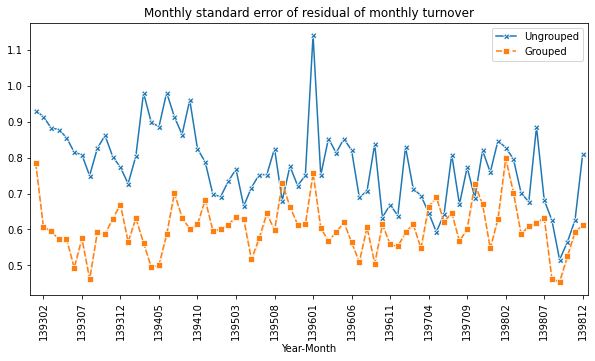
\includegraphics[width=0.85\linewidth]{Output/GroupedResSTD.eps}
		\label{fig:GroupedResSTD}
	\end{figure}
	\item
	برای گروه های کسب و کار متغیر دامی تعریف می کنیم
		\item
		که برای گروه های با انحراف معیار کم در باقی مانده ها برابر یک است
			\item
			بررسی می کنیم که سبب افزایش هم حرکتی می شود
				\item
				برای کنترل و حذف اثر اندازه گروه های کسب و کار، تعداد اعضای هر گروه را هم به صورت کن
\lr{\begin{LTR}
		\begin{table}[htbp]
	\centering
			\resizebox{0.8\textwidth}{!}{
				\centering
				{
\def\sym#1{\ifmmode^{#1}\else\(^{#1}\)\fi}
\begin{tabular}{l*{6}{c}}
\hline\hline
                &\multicolumn{6}{c}{Dependent Variable:  Future Pairs's co-movement}                                              \\\cmidrule(lr){2-7}
                &\multicolumn{1}{c}{(1)}         &\multicolumn{1}{c}{(2)}         &\multicolumn{1}{c}{(3)}         &\multicolumn{1}{c}{(4)}         &\multicolumn{1}{c}{(5)}         &\multicolumn{1}{c}{(6)}         \\
\hline
SameGroup       &   0.0208\sym{***}&   0.0210\sym{***}&                  &                  &   0.0137\sym{***}&   0.0113\sym{**} \\
                &   (7.91)         &   (7.77)         &                  &                  &   (3.73)         &   (3.19)         \\
[1em]
LowTurnoverStd  &                  & 0.000929         &   0.0171\sym{***}&-0.000982         & -0.00107         &  0.00279         \\
                &                  &   (0.84)         &   (3.88)         &  (-0.93)         &  (-1.04)         &   (1.39)         \\
[1em]
$ {\text{LowTurnoverStd} } \times {\text{SameGroup} }  $ &                  &                  &                  &                  &   0.0181\sym{***}&   0.0183\sym{***}\\
                &                  &                  &                  &                  &   (3.65)         &   (3.91)         \\
\hline
Sub-sample      &    Total         &    Total         &SameGroup         &   Others         &    Total         &    Total         \\
Business Group FE&       No         &       No         &       No         &       No         &       No         &      Yes         \\
Observations    &   354209         &   354209         &    43274         &   310935         &   354209         &   354209         \\
\hline\hline  \end{tabular}}

			}
			\label{Turnovercrosssection}
		\end{table}
\end{LTR}}
%\item
%عضویت در گروه کسب و کار سبب هم حرکتی قیمت شرکت ها می شود
%\item
%کانال تاثیر کدام است؟
%\begin{itemize}
%\item
%از متغیر یکسان بودن صنعت به عنوان متغیر ابزاری برای هم بستگی تغییرات
%\lr{turnover}
%استفاده می کنیم تا هم حرکتی قیمت شرکت ها را بررسی کنیم
%\item
%شرایط استفاده از متغیر ابزاری
%\begin{itemize}
%\item
%ارتباط: شرکت های در یک صنعت به همراه یکدیگر معامله می شوند 
%نتایج برآورد 
%\lr{Reduced Form}
%این سوال را پاسخ می دهد
%\item
%برونزایی:
%هم حرکتی شرکت ها نمی تواند صنعت شرکت را تعیین کند
%\item
%\lr{Exclusion restriction}:
%با توجه به نحوه محاسبه هم حرکتی بازده صنعت از آن حذف شده است
%در نتیجه یکسان بودن صنعت دو شرکت نمی تواند سبب هم حرکتی قیمت آن ها شود.
%
%\item \lr{{First Stage} : 
%\begin{equation*}
\begin{split}
\rho(\Delta \text{TurnOver})_{ij,t+1} = & \text{ 	}\beta_0 + \beta_1* \text{SameIndustry} +\beta_3* \rho(\Delta \text{TurnOver}) \\
&+ \sum_{k=1} ^{n} \alpha_k*\text{Control}_{ij,t} + \varepsilon_{ij,t+1}
\end{split}
\end{equation*}}
%\item \lr{{Reduced Form} : 
%\begin{equation*}
\begin{split}
\rho_{ij,t+1} = & \text{ 	}\beta_0 + \beta_1* \text{SameIndustry} +\beta_3* \rho_{ij,t}\\
& + \sum_{k=1} ^{n} \alpha_k*\text{Control}_{ij,t} + \varepsilon_{ij,t+1}
\end{split}
\end{equation*}}
%\item \lr{{Second Stage} : 
%\begin{equation*}
\begin{split}
\rho_{ij,t+1} = & \text{ 	}\beta_0 + \beta_1* IV(\text{SameIndustry}) +\beta_3* \rho_{ij,t} \\
&+ \sum_{k=1} ^{n} \alpha_k*\text{Control}_{ij,t} + \varepsilon_{ij,t+1}
\end{split}
\end{equation*}
%}
%\end{itemize}
%	\lr{
%	\begin{LTR}
%	\begin{table}[htbp]
%			\centering
%			\resizebox{0.75\textwidth}{!}{
%				\centering
%				{
\def\sym#1{\ifmmode^{#1}\else\(^{#1}\)\fi}
\begin{tabular}{l*{3}{c}}
\hline\hline
                    & First Stage         &Reduced form         &Second Stage         \\
                    &\multicolumn{1}{c}{(1)}         &\multicolumn{1}{c}{(2)}         &\multicolumn{1}{c}{(3)}         \\
\hline
SameIndustry        &      0.0285\sym{***}&     0.00133         &                     \\
                    &     (14.59)         &      (1.09)         &                     \\
[1em]
 $ {\rho(\Delta \text{TurnOver})_{t+1}} $ &                     &                     &      0.0805\sym{*}  \\
                    &                     &                     &      (2.45)         \\
[1em]
Same Group          &      0.0242\sym{***}&      0.0167\sym{***}&      0.0174\sym{***}\\
                    &     (10.73)         &      (9.72)         &     (10.40)         \\
[1em]
SameSize            &      0.0332\sym{***}&      0.0158\sym{***}&      0.0160\sym{***}\\
                    &      (3.47)         &      (5.67)         &      (9.18)         \\
[1em]
SameBookToMarket    &      0.0183\sym{***}&     0.00711\sym{***}&     0.00554\sym{***}\\
                    &      (4.38)         &      (4.46)         &      (4.48)         \\
[1em]
CrossOwnership      &      0.0393\sym{***}&      0.0172         &      0.0165\sym{*}  \\
                    &      (3.52)         &      (1.59)         &      (2.13)         \\
\hline
Observations        &     1341445         &     1665996         &     1447736         \\
Method              &          FE         &          FE         &        2sls         \\
Group FE            &         Yes         &         Yes         &         Yes         \\
Pair Size Control   &         Yes         &         Yes         &         Yes         \\
Lag of Dep. Var.    &         Yes         &         Yes         &         Yes         \\
$ R^2$              &     0.00231         &     0.00111         &                     \\
\hline\hline
\multicolumn{4}{l}{\footnotesize \textit{t} statistics in parentheses}\\
\multicolumn{4}{l}{\footnotesize \sym{*} \(p<0.05\), \sym{**} \(p<0.01\), \sym{***} \(p<0.001\)}\\
\end{tabular}
}

%			}
%			\label{TurnIv}
%		\end{table}
%		\end{LTR}
%		}
%\end{itemize}
%حال برای بررسی نهایی به عنوان متغییر کنترلی همبستگی تغییرات 
%\lr{turnover}
%جفت ها را به مدل اصلی اضافه می کنیم
%
%		
%	\begin{itemize}
%		\item 
%	برای رفع مشکل 
%	\lr{reverse casulity}
%	از لگ هم حرکتی قیمت شرکت ها استفاده می کنیم
%	\item
%	نتایج در جدول 
%			\ref{BigBusinessGroup}
%			نشان داده شده است
%			
%				\begin{itemize}
%				\item
%				در دو ستون اول هم بستگی تغییرات 
%				\lr{turnover}
%				را به مدل اضافه کرده ایم
%				\item
%				افزایش هم بستگی تغییرات
%				\lr{turnover}
%				در شرکت ها سبب افزایش هم حرکتی قیمت شرکت ها می شود
%				\item
%				در جفت های عضو یک گروه کسب و کار نیز تاثیر هم حرکتی تغییرات  
%				\lr{turnover}
%				بیشتر است
%				\end{itemize}
%					\item 
%								در ادامه انتظار داریم گروه های بزرگ کسب و کار به دلیل آگاهی فعالان بازار در رابطه با وجود این گروه ها، به همراه یکدیگر معامله شوند	
%							\begin{itemize}
%								
%								\item 
%								برای این منظور گروه های کسب و کار را براساس تعداد اعضا دسته بندی کردیم و  گروه های بالاتر از میانه را گروه های بزرگ در نظر گرفتیم.
%								\item 
%								انتظار داریم هم حرکتی جفت های در گروه های کسب و کار بزرگ بیشتر از جفت های دیگر باشد
%								\item
%								از طرفی تاثیر معاملات هم زمان نیز در این گروه ها باید بیشتر از گروه های کوچک باشد
%								\item
%								در گروه های کسب و کار بزرگ هم حرکتی در تغییرات 
%								\lr{turnover}
%								توضیح دهندگی بیشتری نسبت به دیگر گروه ها داشته باشد
%								\item
%								نتایج برآورد در جدول
%								\ref{BigBusinessGroup}
%								نشان داده شده است
%							
%								\item
%								در گروه های بزرگ هم بستگی تغییرات 
%								\lr{turnover}
%								تاثیر بیشتری بر روی هم بستگی دارد
%								\item
%								در صورتی که در دیگر گروه ها تاثیر هم بستگی در تغییرات 
%								\lr{turnover}
%								کمتر است
%								
%								
%							\end{itemize}
%	\end{itemize}
%	
%	
%		\begin{LTR}
%						\lr{		\begin{table}[htbp]
%								\centering
%								\caption{heading}
%								\label{BigBusinessGroup}
%								\resizebox{\textwidth}{!}{
%									{
\def\sym#1{\ifmmode^{#1}\else\(^{#1}\)\fi}
\begin{tabular}{l*{5}{c}}
\hline\hline
                &\multicolumn{5}{c}{Dependent Variable: Future Pairs's co-movement}                            \\\cmidrule(lr){2-6}
                &\multicolumn{1}{c}{(1)}         &\multicolumn{1}{c}{(2)}         &\multicolumn{1}{c}{(3)}         &\multicolumn{1}{c}{(4)}         &\multicolumn{1}{c}{(5)}         \\
\hline
Same Group      &   0.0263\sym{***}&   0.0250\sym{***}&   0.0380\sym{***}&   0.0244\sym{**} &   0.0256\sym{***}\\
                &   (3.79)         &   (3.55)         &   (5.82)         &   (3.33)         &   (4.02)         \\
[1em]
 $ {\rho\_t(\text{Turnover})} $ &  0.00475\sym{***}&  0.00419\sym{***}&  0.00474\sym{***}&  0.00383\sym{***}&  0.00493\sym{***}\\
                &   (9.75)         &   (8.55)         &   (4.65)         &   (4.64)         &   (4.66)         \\
[1em]
 $ {\rho\_t} $   &   0.0249\sym{***}&   0.0248\sym{***}&   0.0248\sym{***}&   0.0252\sym{***}&   0.0243\sym{***}\\
                &  (11.12)         &  (11.10)         &  (11.03)         &  (10.64)         &   (8.58)         \\
[1em]
$ {\text{SameGroup} \times  {\rho\_t(\text{Turnover})} } $ &                  &   0.0172\sym{***}& -0.00936         &   0.0224\sym{***}&  -0.0114         \\
                &                  &   (3.63)         &  (-0.84)         &   (4.42)         &  (-1.04)         \\
[1em]
BigGroup        &                  &                  & -0.00186         &                  &                  \\
                &                  &                  &  (-1.99)         &                  &                  \\
[1em]
$ {\text{BigGroup} } \times {\text{SameGroup} }  $ &                  &                  &  -0.0151\sym{*}  &                  &                  \\
                &                  &                  &  (-2.43)         &                  &                  \\
[1em]
$ {\text{BigGroup} } \times  {\rho\_t(\text{Turnover})}  $ &                  &                  &-0.000833         &                  &                  \\
                &                  &                  &  (-0.53)         &                  &                  \\
[1em]
$ {\text{BigGroup}}\times{\text{SameGroup}}\times  {\rho\_t(\text{Turnover})}$ &                  &                  &   0.0317\sym{*}  &                  &                  \\
                &                  &                  &   (2.64)         &                  &                  \\
\hline
Observations    &  1459585         &  1459585         &  1459585         &   957316         &   502269         \\
Controls        &      Yes         &      Yes         &      Yes         &      Yes         &      Yes         \\
Pari Size FE    &      Yes         &      Yes         &      Yes         &      Yes         &      Yes         \\
SubSample       &      All         &      All         &      All         &Big Groups         &   Others         \\
$ R^2$          &  0.00244         &  0.00255         &  0.00302         &  0.00307         &  0.00396         \\
\hline\hline
\multicolumn{6}{l}{\footnotesize \textit{t} statistics in parentheses}\\
\multicolumn{6}{l}{\footnotesize \sym{*} \(p<0.05\), \sym{**} \(p<0.01\), \sym{***} \(p<0.001\)}\\
\end{tabular}
}

%								}
%						\end{table}}
%					\end{LTR}
\end{itemize}

\FloatBarrier




\FloatBarrier







\FloatBarrier


 \subsection{\lr{Institutional Imbalance}}
 \begin{itemize}
 	\item 
 	در قسمت قبل نشان دادیم که شرکت های درون گروه به همراه هم حرکت می شوند و این امر سبب می شود تا هم حرکتی قیمتی نیز با یدیگر داشته باشند
 	\item
 	حال بررسی می کنیم تا شرکت ها در یک جهت نیز معامله شوند
 	\item
 	یکی از ملاک های مورد استفاده در ادبیات برای بررسی رفتار معامله گران  ناترازی خرید و فروش است
 	
 	\lr{\cite{seasholes2007predictable}}
 
 		\begin{equation}
 			Imbalance_{ins} = \frac{Buy_{ins} - Sell_{ins}}{Buy_{ins} + Sell_{ins}}
 		\end{equation}

 	\item 
 	در سطح ماه ملاک ناترازی خرید و فروش را تعریف می کنیم
 	\item 
 	که در عبارت های ذکر شده مجموع خرید و فروش در سطح یک ماه در نظر گرفته شده است
 	\item 
 	مشخصات آماری ناترازی حقوقی در جدول 
 	\ref{tab:ImbalanceInsMeanSummary}
 	بیان شده است
  	\begin{LTR}
 	\lr{\begin{table}[htbp]
 			\centering
 			\caption{text}
 			\resizebox{0.75\textwidth}{!}{
 				\begin{tabular}{lrrrrrrrr}
\toprule
{} &  Group $\times$ Month &   mean &    std &  min &    25\% &    50\% &    75\% &  max \\
Grouped   &                       &        &        &      &        &        &        &      \\
\midrule
Ungrouped &                 20197 &  0.010 &  0.630 & -1.0 & -0.474 &  0.016 &  0.479 &  1.0 \\
Grouped   &                 12021 & -0.041 &  0.581 & -1.0 & -0.462 & -0.009 &  0.341 &  1.0 \\
\bottomrule
\end{tabular}

 			}
 			\label{tab:ImbalanceInsMeanSummary}
 	\end{table}}
 \end{LTR}

 \end{itemize}
 \FloatBarrier
 
 \begin{itemize}
 	\item 
 	اگر شرکت های در یک گروه کسب و کار به همراه یکدیگر معامله شوند انتظار داریم تا انحراف معیار ناترازی خرید و فروش  حقوقی در گروه کمتر از شرکت های بیرون گروه باشد
 	\item 
 	انحراف معیار ناترازی حقوقی در شرکت های درون گروه و بیرون گروه را بررسی کرده ایم
 		\item 
 	جدول 
 		\ref{tab:ImbalanceInsStdSummary}
 	و
 	نتایج را نشان می دهد
 	\begin{LTR}
 		\lr{\begin{table}[htbp]
 				\centering
 				\caption{text}
 				\resizebox{0.75\textwidth}{!}{
 					\begin{tabular}{lcccccccc}
\toprule
{} &  Group $\times$ Month &   mean &    std &   min &    25\% &    50\% &    75\% &    max \\
Grouped   &                       &        &        &       &        &        &        &        \\
\midrule
Ungrouped &                    72 &  0.624 &  0.054 &  0.48 &  0.601 &  0.631 &  0.655 &  0.735 \\
Grouped   &                  2057 &  0.503 &  0.251 &  0.00 &  0.337 &  0.503 &  0.647 &  1.414 \\
\bottomrule
\end{tabular}

 				}
 				\label{tab:ImbalanceInsStdSummary}%
 		\end{table}}
 	\end{LTR}

 		\item 
 	به صورت متوسط انحراف معیار ناترازی در شرکت های درون گروه از شرکت های بیرون گروه کمتر است	
 	
 	\item 
 	در شکل 
 	\ref{fig:GroupedInsSTD}
 	سری زمانی میانگین انحراف معیار ناترازی شرکت ها در گروه ها و بیرون گروه نشان داده شده است
 	\begin{figure}[htbp]
 		\centering
 		\caption{text}
 		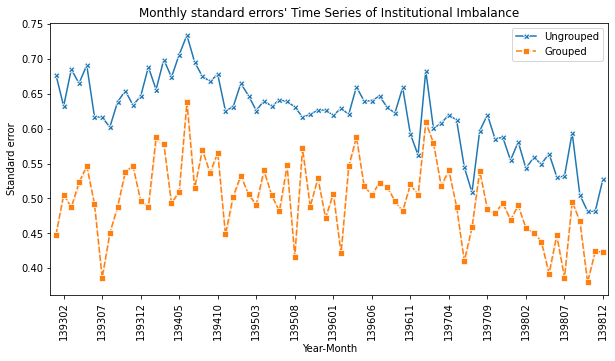
\includegraphics[width=0.85\linewidth]{Output/GroupedInsSTD.eps}
 		\label{fig:GroupedInsSTD}
 	\end{figure}

 	\item 
 	به صورت متوسط انحراف معیار نا ترازی برای حقوقی ها 12\%
 	از شرکت های بیرون گروه کمتر است. (از لحاظ آماری هم این اختلاف معنا دار است)
 	
 \end{itemize}
  

\begin{itemize}
	\item 
	همانطور که انتظار داشتیم در گروه های کسب و کار انحراف معیار نا ترازی کم است
	\item 
	حال باید نشان دهیم که جفت های حاضر  در گروه های کسب و کار با انحراف معیار کمتر، هم حرکتی بالاتری نیز دارند
	\item 
	برای این هدف متغیر دامی 
	\textbf{Imbalance std}
	را برای گروه هایی که انحراف معیار ناترازی حقوقی برای آن ها از میانه کمتر است تعریف می کنیم
%	\item 
%	مدل زیر را با استفاده از روش مدل 
%	\ref{model1}
%	برآورد می کنیم
%	\textsl{}\begin{equation}
\begin{split}
\rho_{ij,t+1} = & \text{ 	}\beta_0 + \beta_1* \text{FCA}^*_{ij,t} + \beta_2* \text{SameGroup}_{ij} + \beta_3 * \text{Low Imbalance std} \\
& +\beta_4* \text{Low Imbalance std} \times \text{SameGroup}_{ij}  \\
& +\beta_5* \text{FCA}^*_{ij,t} \times \text{SameGroup}_{ij}  \\
& +\beta_6* \text{Low Imbalance std} \times \text{FCA}^*_{ij,t}  \\
 & 	+\beta_4* \text{Low Imbalance std} \times \text{SameGroup}_{ij} \times \text{FCA}^*_{ij,t}   \\
  & + \sum_{k=1} ^{n} \alpha_k*\text{Control}_{ij,t} + \varepsilon_{ij,t+1}
\end{split}
\label{model1}
\end{equation}
	\item 
	انتظار داریم جفت های حاضر در گروه های با انحراف معیار کم هم حرکتی بیشتری داشته باشند
	
\end{itemize}

\begin{itemize}
	\item 
	نتایج در جدول
	\ref{Imbalance}
	آورده شده است
	\begin{LTR}
		\lr{\begin{table}[htbp]
		\centering
		\caption{text}
		\label{Imbalance}
		\resizebox{\textwidth}{!}{
			{
\def\sym#1{\ifmmode^{#1}\else\(^{#1}\)\fi}
\begin{tabular}{l*{6}{c}}
\hline\hline
                    &\multicolumn{6}{c}{Dependent Variable:  Future Pairs's Comovement}                                                                 \\\cmidrule(lr){2-7}
                    &\multicolumn{1}{c}{(1)}         &\multicolumn{1}{c}{(2)}         &\multicolumn{1}{c}{(3)}         &\multicolumn{1}{c}{(4)}         &\multicolumn{1}{c}{(5)}         &\multicolumn{1}{c}{(6)}         \\
\hline
SameGroup           &      0.0208\sym{***}&      0.0206\sym{***}&                     &                     &     0.00619         &     0.00630\sym{*}  \\
                    &      (7.91)         &      (7.94)         &                     &                     &      (1.95)         &      (2.04)         \\
[1em]
LowImbalanceStd     &                     &    -0.00144         &      0.0282\sym{***}&    -0.00724\sym{***}&    -0.00610\sym{***}&    -0.00267         \\
                    &                     &     (-1.15)         &      (6.06)         &     (-5.74)         &     (-4.87)         &     (-1.85)         \\
[1em]
 $ \text{LowImbalanceStd} \times {\text{SameGroup} } $ &                     &                     &                     &                     &      0.0358\sym{***}&      0.0325\sym{***}\\
                    &                     &                     &                     &                     &      (8.57)         &      (7.48)         \\
\hline
Sub-sample          &       Total         &       Total         &   SameGroup         &      Others         &       Total         &       Total         \\
Business Group FE   &          No         &          No         &          No         &          No         &          No         &         Yes         \\
Observations        &      354209         &      354209         &       43274         &      310935         &      354209         &      354209         \\
\hline\hline
\multicolumn{7}{l}{\footnotesize \textit{t} statistics in parentheses}\\
\multicolumn{7}{l}{\footnotesize \sym{*} \(p<0.05\), \sym{**} \(p<0.01\), \sym{***} \(p<0.001\)}\\
\end{tabular}
}

		}
	\end{table}}
	\end{LTR}
\begin{itemize}
	\item 
	همچنان جفت های در یک گروه کسب و کار هم حرکتی بیشتری دارند
	\item 
	اگر جفت های در یک گروه کسب و کار، در گروه های با انحراف معیار کم باشند $ 2.4\% $ هم حرکتی آن ها افزایش پیدا می کند
	(میانگین هم حرکتی تقریبا $ 1.6 \%$ است )

	
\end{itemize}
\end{itemize}

\FloatBarrier



 \section{Conclusion}
\begin{itemize}
	\item 
	نحوه محاسبه مالکیت مشترک را بهبود دادیم
	\item 
	مالکیت مشترک دارای اهمیت است 
	\item 
	گروه های کسب و کار داری اهمیت است
	\item 
	گروه کسب و کار از مالکیت مشترک اهمیت بالاتری دارد
	\item 
	گروه های کسب و کار از طریق معامله هم زمان بر روی هم حرکتی تاثیر می گذارند.
	
	
\end{itemize}


\newpage
\begin{LTR}

\footnotesize{
	\bibliographystyle{apalike}
	\bibliography{Ref}
}
\end{LTR}

%
\begin{appendices}
\section{\lr{Modified Anton's measure}}
\label{ModifiedMeasure}
\begin{itemize}
	\item 
	فرمول استفاده شده در مقاله
	\lr{\cite{AntonPolk}}
		\begin{equation}
		\text{Overlap}_{Sum}(i, j) = \frac{\sum_{f = 1}^{F} (S^f_{i,t}P_{i,t}+S^f_{j,t}P_{j,t})}{S_{i,t}P{i,t} + S_{j,t}P{j,t}}
		\label{Sum}
	\end{equation}
	\item 
	این فرمول توزیع مالکیت را در نظر نمیگیرد و فقط جمع ساده است
	\item
وزن دهی دوباره انجام دادیم و دو فرمول زیر را پیشنهاد می دهیم	
	\item

\begin{equation}
	\text{Overlap}_{Sqrt}(i, j) =  [\frac{\sum_{f =1}^{F}(\sqrt{S^f_{i,t}P_{i,t}}+\sqrt{S^f_{j,t}P_{j,t}})}{\sqrt{S_{i,t}P{i,t}} + \sqrt{S_{j,t}P{j,t}}}]^2 
	\label{sqrt}
\end{equation}

\begin{equation}
	\text{Overlap}_{Quadratic}(i, j) =  [{\frac{\sum_{f = 1}^{F}[(S^f_{i,t}P_{i,t})^2+(S^f_{j,t}P_{j,t})^2]}{(S_{i,t}P{i,t})^2 + (S_{j,t}P{j,t})^2}}]^{-1}
	\label{Quadratic}
\end{equation}
	\item
تفسیر این دو ملاک عبارت است از این که در صورت تقسیم دو شرکت به صورت مساوی بین n مالک، این ملاک عدد n را نشان می دهد
\LR{\footnote{ \tiny
	Each holder owns $ 1/n $ of each firm ,Firm's market cap is $ \alpha_1 $ and $ \alpha_2 $, So for each holder of firms we have $ S^f_{i,t}P_{i,t} = \alpha_i/n $\\
	$
	[  \frac{\sum_{f=1}^{n} \sqrt{\alpha_1/n}+\sum_{f=1}^{n} \sqrt{\alpha_2/n}}{\sqrt{\alpha_1} + \sqrt{\alpha_2}}]^2 
	= [\frac{\sqrt{n}(\sqrt{\alpha_1} +\sqrt{\alpha_2 })}{\sqrt{\alpha_1} + \sqrt{\alpha_2}}]^2 = n $
	\\
	$
	[\frac{\sum_{f=1}^{n} {(\alpha_1/n)^2}+\sum_{f=1}^{n} {(\alpha_2/n)^2}}{\alpha_1^2 +{\alpha_2}^2}]^{-1} = [\frac{{\alpha_1^2 + \alpha_2^2 }}{n(\alpha_1^2 + \alpha_2^2)}]^{-1} = n
	$
}}
	\item
در واقع یعنی تعداد مالک مشترک مساوی دو شرکت را تولید می کند
\end{itemize}

\begin{itemize}
	\item 
	مثال عددی برای مقایسه دو ملاک معرفی شده
	\begin{itemize}
		\item 
		دو شرکت x و y با یک مالک مشترک با مالکیت 
		 $ \alpha $ 
		 و
		  $ \beta $
		از مارکت کپ دو شرکت با ارزش یکسان.
		شکل 
		\ref{gExample1}
		\begin{itemize}
			\item 
			برای سادگی فرق می کنیم
			($ \alpha + \beta  = 100$)
			\item شکل مثال
				\begin{figure}[htbp]
				\centering
				\caption{\lr{ Numeric example 1} }
				\label{gExample1}
				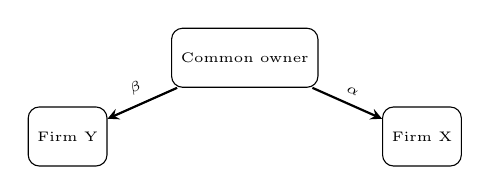
\begin{tikzpicture}[node distance=1cm]
					
					\node (Firm) [startstop3] {\tiny Firm X};
					\node (Firm2) [startstop3,right of = Firm  , xshift=-5.5cm ] {\tiny Firm Y};
					\node (Owner) [startstop3,right of = Firm , yshift=1cm , xshift=-3.25cm ] {\tiny Common owner };
					
					
					\draw[arrow] (Owner) -- node[sloped, anchor=center, above] {\tiny $ \alpha $} (Firm) ;
					
					\draw[arrow] (Owner) -- node[sloped, anchor=center, above] {\tiny $ \beta $} (Firm2) ;
					%
					%\node() at (3,0)
					%    {$ \alpha + \beta = 100 $}; 
				\end{tikzpicture}
			\end{figure}\bigskip
\item
شکل 
\ref{example1Results}
نتایج محاسبات را نشان می دهد
\item
\begin{figure}[htbp]
	\caption{ \lr{Comparison of three measure for common ownership}}
	\label{example1Results}
	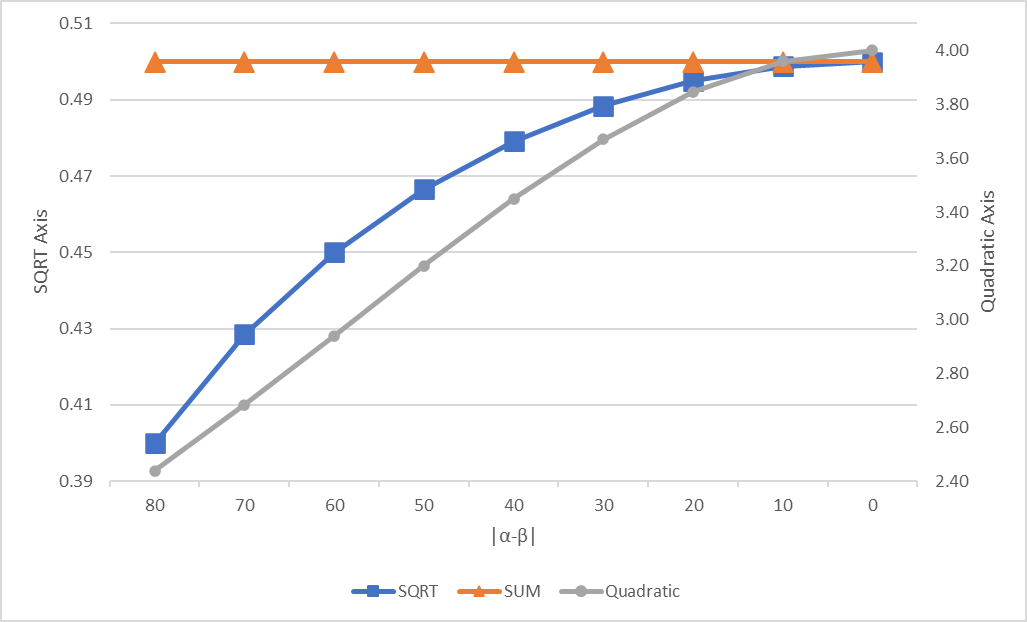
\includegraphics[width=0.47\linewidth]{Elements/1.png}
	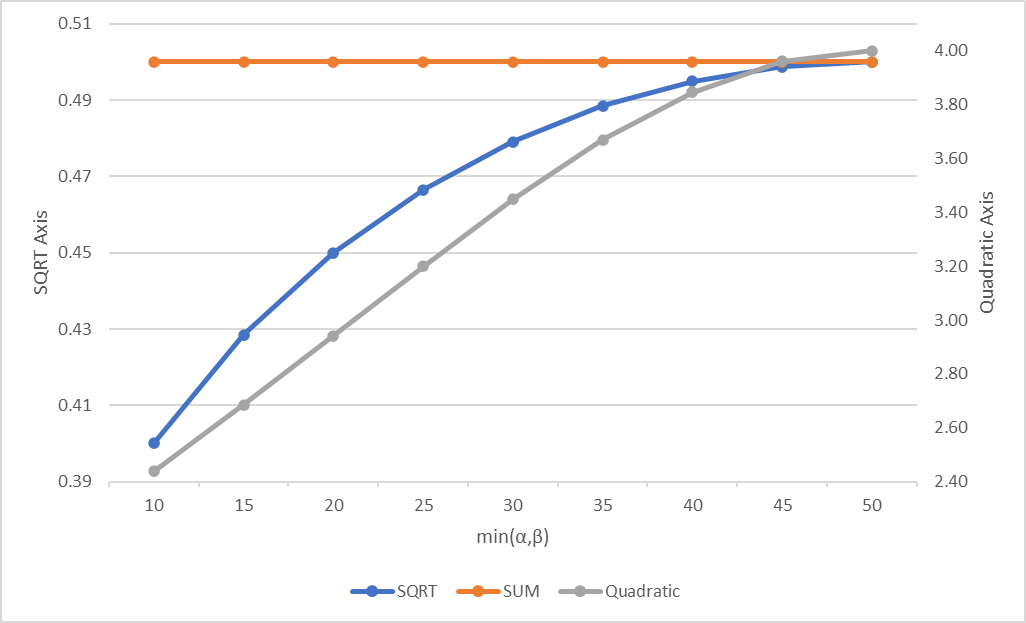
\includegraphics[width=0.47\linewidth]{Elements/2.png}
\end{figure}
\item
ملاک اصلی برای هر توزیعی ثابت است ولی دو ملاک معرفی شده تفاوت را ایجاد کرده است
\item
مالکیت مشترک در حال 50-50 بیشترین و در حال 10-90 کمترین حالت ممکن است 


\end{itemize}
\item 
		حال در مثال قبل فرض کنید سه مالک مشترک داریم که در برای مالک 1 مالکیت در شرکت x و y عبارت است از 
		$\alpha_1$ 
		و
		$\beta_1$
		
		\begin{itemize}
			\item 
			شکل مثال
			\begin{figure}[htbp]  \centering
				\caption{ Numeric example 2}
				\label{gExample2}
				\centering
				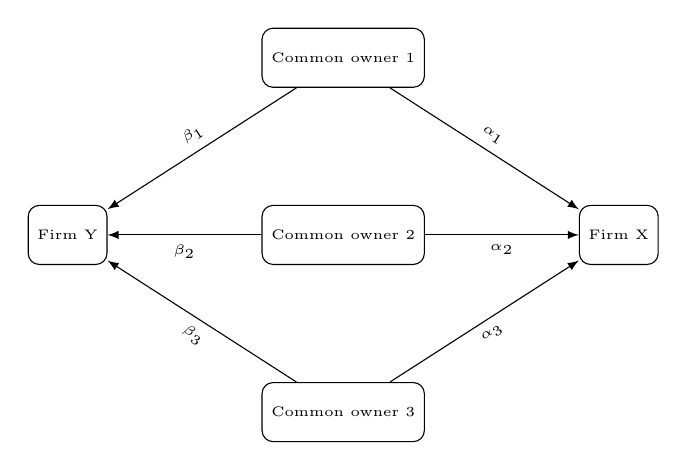
\begin{tikzpicture}[node distance=1cm]
					
					
					\node (Firm) [startstop3] {\tiny Firm X};
					\node (Firm2) [startstop3,right of = Firm , yshift=0cm , xshift=-8cm ] {\tiny Firm Y};
					
					\node (Owner) [startstop3,above of = Firm , yshift=1.25cm , xshift=-3.5cm ] {\tiny Common owner 1 };
					
					
					\node (Owner2) [startstop3,right of = Firm , yshift= 0 , xshift=-4.5cm ] {\tiny Common owner 2 };
					
					\node (Owner3) [startstop3,below of = Firm , yshift=-1.25cm , xshift=-3.5cm ] {\tiny Common owner 3 };
					
					
					
					
					
					\draw [-latex] (Owner) to [bend right =0]  node[sloped, anchor=center, above] {\tiny $ \beta_1 $} (Firm2);
					
					\draw [-latex] (Owner) to [bend left =0]  node[sloped, anchor=center, above] {\tiny $ \alpha_1 $} (Firm);
					
					
					
					\draw [-latex] (Owner2) to [bend right =0]  node[sloped, anchor=center, below] {\tiny $ \beta_2 $} (Firm2);
					
					\draw [-latex] (Owner2) to [bend left =0]  node[sloped, anchor=center, below] {\tiny $ \alpha_2 $} (Firm);
					
					
					
					\draw [-latex] (Owner3) to [bend left =0]  node[sloped, anchor=center, below] {\tiny$ \beta_3 $} (Firm2);
					
					\draw [-latex] (Owner3) to [bend right =0]  node[sloped, anchor=center, below] {\tiny $ \alpha_3 $} (Firm);
					
					
					
				\end{tikzpicture}
			\end{figure}
			\item 
			نتایح در 
			\ref{Example2}
			نشان داده شده است
			\begin{LTR}
				\lr{\begin{table}[htbp]
				\centering
				\caption{ text}
				\label{Example2}
				\resizebox{1\textwidth}{!}
				{
					    \begin{tabular}{cccccccc}
    \hline\hline
        Ownership  & Type I & Type II & Type III & Type IV & Type V & Type VI & Type VII \\
          \hline
    $ \alpha_1 $    & 1/3 &20      &  10   & 20    & 10    & 5     & 1  \\
    $ \beta_1 $    & 1/3  & 10    & 10   & 20    & 10    & 5     & 1  \\
    $ \alpha_2 $    & 1/3  & 10    & 80    & 20    & 10    & 5     & 1 \\
    $ \beta_2 $    & 1/3  & 20    & 80    & 20    & 10    & 5     & 1  \\
    $ \alpha_3 $    & 1/3  & 70    & 10    & 20    & 10    & 5     & 1 \\
    $ \beta_3 $    & 1/3  & 70    & 10   & 20    & 10    & 5     & 1  \\
    \hline
    SQRT  & 3     &  2.56  & 2.33 & 1.8   & 0.9   & 0.45  & 0.09 \\
    SUM   & 1     & 1     & 1     & 0.6   & 0.3   & 0.15  & 0.03 \\
    Quadratic & 3     & 1.85  & 1.52  & 8.33  & 33.33 & 133.33 & 3333.33 \\
 
    \hline\hline
    \end{tabular}%
				}
			\end{table}}
			\end{LTR}
			\item 
			برای مالکیت های برابر تمام مارکت کپ تو شرکت نتایج با قبل یکسان است
			\item 
			ستون اول هم تفسیر ملاک را نشان می دهد که در صورت تقسیم شرکت به 3 مالک، عدد برابر 3 است
			\item 
			برای مالکیت های کمتر از 100 درصد ملاک درجه 2 مقادیر غیر واقعی تولید می کند
			\item 
			برای همین از ملاک جذری استفاده می کنیم
			
			
		\end{itemize}
		\item 
		حال فرض اصلی که ارزش بازاری دو شرکت برابر است را کنار می گذاریم برای مثال دو شرکت را با دو مالک مشترک در حالت های مختلف بررسی می کنیم

		
		\begin{itemize}
			\item 
			شکل 
			 \ref{sqrtMarket}
			 و
			  \ref{sumMarket}
			  نتایج را برای جمع ثابت مالکیت برای سه حالت توزیع مختلف رسم شده است
			  
			\item 
		\begin{LTR}
			\lr{	\begin{figure}[htbp]
				\centering
				\caption{ SQRT measure for fixed aggregate ownership on different relative market cap ratios}
				\label{sqrtMarket}
				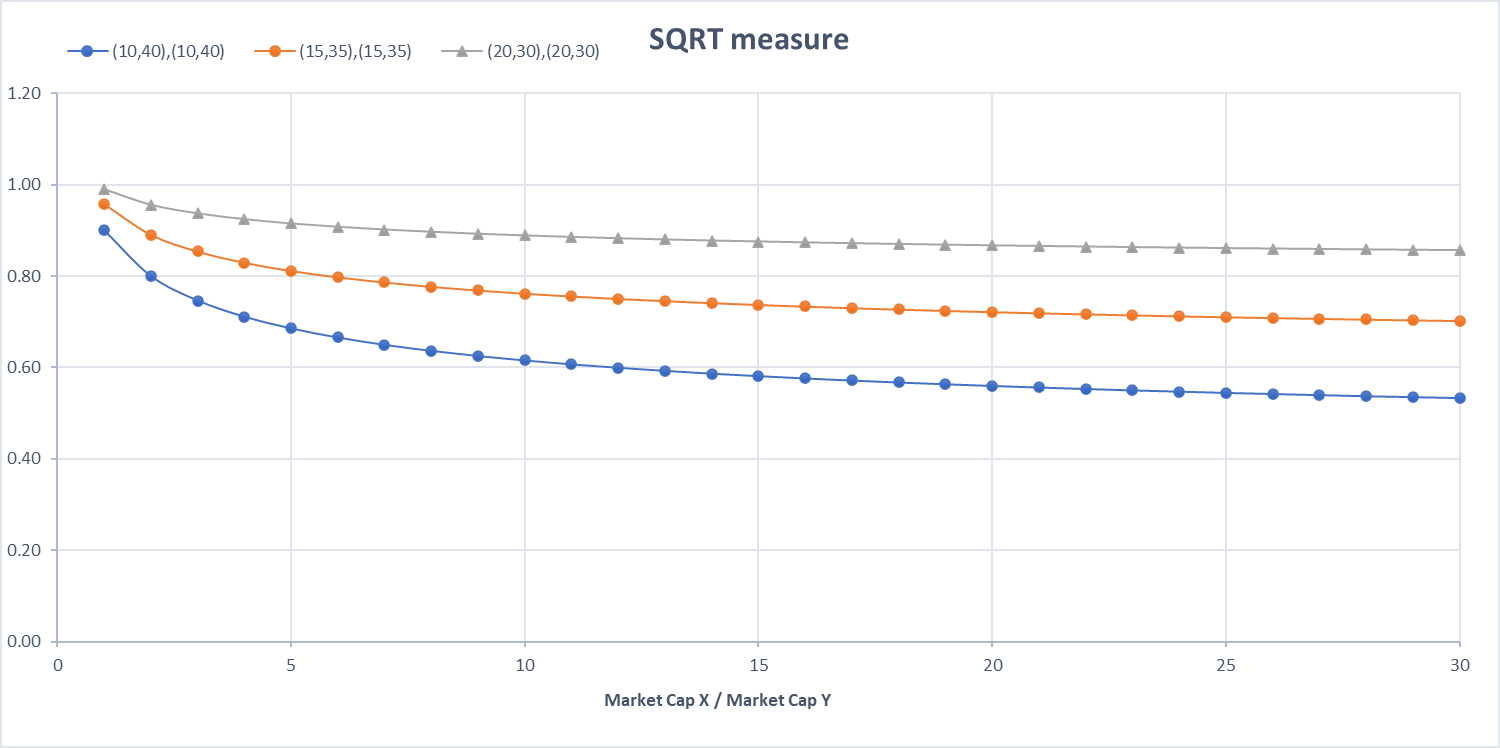
\includegraphics[width=0.85\linewidth]{Elements/3.png}
			\end{figure}
			\begin{figure}[htbp]
				\centering
				\caption{ Sum measure for fixed aggregate ownership on different relative market cap ratios}
				\label{sumMarket}
				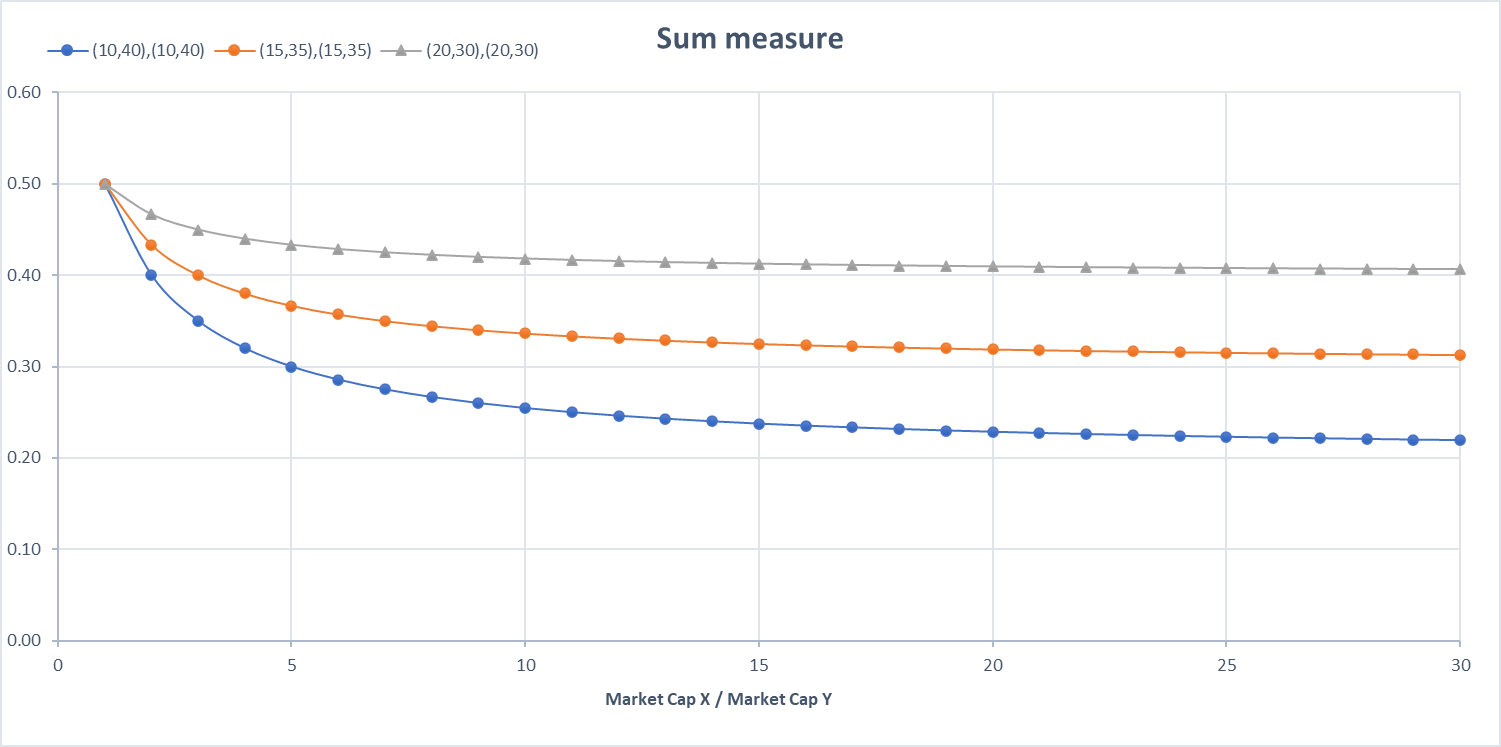
\includegraphics[width=0.85\linewidth]{Elements/4.png}
			\end{figure}}
		\end{LTR}
			\item 
			جدول 
			\ref{marketcap}
			نتایج محاسبات را نشان داده است.
			
			\item 
			\begin{LTR}
				\lr{\begin{table}[htbp]
						\centering
						\caption{text }
						\label{marketcap}
						\resizebox{!}{!}
						{
							          \scriptsize
    \begin{tabular}{ccccccc}
    \hline\hline
  & \multicolumn{6}{c}{\tiny($ \alpha_1 $,$ \beta_1 $),($ \alpha_2 $,$ \beta_2 $) }\\ \cmidrule(lr){2-7}
               & \multicolumn{2}{c}{\tiny(10,40),(10,40)} & \multicolumn{2}{c}{\tiny(15,35),(15,35)} & \multicolumn{2}{c}{\tiny(20,30),(20,30)} \\ \cmidrule(lr){2-3}\cmidrule(lr){4-5}\cmidrule(lr){6-7}
    \tiny $ \frac{\text{MarketCap}_x}{\text{MarketCap}_y} $     &\tiny SQRT  & \tiny SUM   &\tiny SQRT  &\tiny SUM   &\tiny SQRT  &\tiny SUM \\ 
     \hline\addlinespace

         1     & 0.90  & 0.50  & 0.96  & 0.50  & 0.99  & 0.50 \\
         2     & 0.80  & 0.40  & 0.89  & 0.43  & 0.96  & 0.47 \\
         3     & 0.75  & 0.35  & 0.85  & 0.40  & 0.94  & 0.45 \\
         4     & 0.71  & 0.32  & 0.83  & 0.38  & 0.92  & 0.44 \\
         5     & 0.69  & 0.30  & 0.81  & 0.37  & 0.91  & 0.43 \\
         6     & 0.67  & 0.29  & 0.80  & 0.36  & 0.91  & 0.43 \\
         7     & 0.65  & 0.28  & 0.79  & 0.35  & 0.90  & 0.43 \\
         8     & 0.64  & 0.27  & 0.78  & 0.34  & 0.90  & 0.42 \\
         9     & 0.63  & 0.26  & 0.77  & 0.34  & 0.89  & 0.42 \\
         10    & 0.62  & 0.25  & 0.76  & 0.34  & 0.89  & 0.42 \\
     
    \hline\hline
    \end{tabular}
						}
			\end{table}}
			\end{LTR}
			\item
			ملاک وزن دهی جذری به دلیل تغییرات بهتر و مقادیر معقول برای مقادیر کم مالکیت مشترک انتخاب شده است
		\end{itemize}

		
		
	\end{itemize}
\end{itemize}













\subsection{\lr{Common Ownership measure}}
\begin{itemize}
	\item 
	برآورد مدل اصلی برای دو نوع اندازه گیری مالکیت مشترک
	\item 
	به شیوه قبلی
	\item 
	در نظر گرفتن توزیع سبب کاهش معناداری می شود که نشان می دهد بین حالت های مختلف توزیع تفاوت وجود دارد
	\item
	اثر در اندازه گیری جمع ساده بیش از اندازه برآور می شد
	
\end{itemize}

{\begin{table}[htbp]
		%	\centering
		\caption{Connected Co-movement}
		\label{mresult2Polk}
		\resizebox{1\textwidth}{!}{
			\begin{LTR}
				\lr{{
\def\sym#1{\ifmmode^{#1}\else\(^{#1}\)\fi}
\begin{tabular}{l*{8}{c}}
\hline\hline
                &\multicolumn{8}{c}{Dependent Variable: Future Monthly Correlation of 4F+Industry Residuals}                                                            \\\cmidrule(lr){2-9}
                &\multicolumn{1}{c}{(1)}         &\multicolumn{1}{c}{(2)}         &\multicolumn{1}{c}{(3)}         &\multicolumn{1}{c}{(4)}         &\multicolumn{1}{c}{(5)}         &\multicolumn{1}{c}{(6)}         &\multicolumn{1}{c}{(7)}         &\multicolumn{1}{c}{(8)}         \\
\hline
Common Ownership Measure&  0.00370\sym{***}&  0.00325\sym{***}&  0.00155\sym{*}  &  0.00109         & 0.000333         &-0.000105         & 0.000550         & 0.000283         \\
                &   (5.58)         &   (4.97)         &   (2.61)         &   (1.84)         &   (0.54)         &  (-0.17)         &   (1.07)         &   (0.58)         \\
[1em]
SameGroup       &                  &                  &   0.0229\sym{***}&   0.0234\sym{***}&   0.0100\sym{**} &   0.0103\sym{**} &  0.00626         &  0.00668         \\
                &                  &                  &   (7.89)         &   (7.93)         &   (3.26)         &   (3.17)         &   (1.79)         &   (1.79)         \\
[1em]
 $ \text{\small Common Ownership Measure} \times {\text{SameGroup} }$ &                  &                  &                  &                  &   0.0134\sym{***}&   0.0135\sym{***}&   0.0127\sym{***}&   0.0126\sym{***}\\
                &                  &                  &                  &                  &   (9.47)         &  (10.65)         &   (9.23)         &   (9.71)         \\
\hline
Observations    &   398818         &   398818         &   398818         &   398818         &   398818         &   398818         &   398818         &   398818         \\
Group FE        &       No         &       No         &       No         &       No         &       No         &       No         &      Yes         &      Yes         \\
Measurement     &      Sum         &      Sum         &      Sum         &      Sum         &      Sum         &     SQRT         &      Sum         &     SQRT         \\
$ R^2 $         &  0.00433         &  0.00427         &  0.00518         &  0.00515         &  0.00554         &  0.00551         &   0.0182         &   0.0182         \\
\hline\hline
\multicolumn{9}{l}{\footnotesize \textit{t} statistics in parentheses}\\
\multicolumn{9}{l}{\footnotesize \sym{*} \(p<0.05\), \sym{**} \(p<0.01\), \sym{***} \(p<0.001\)}\\
\end{tabular}
}
}
			\end{LTR}
		}
\end{table}}

\FloatBarrier





\FloatBarrier



\section{\lr{Overview of Business Groups in Tehran Stock Exchange}} \label{BGDef}

\begin{itemize}
	\item 
	گروه های کسب و کار در کشور های در حال توسعه و توسعه یافته وجود دارد
	
	\lr{\cite{Khanna2007}}
	\item 
	گروه کسب و کار مجموعه ای از شرکت های به هم پیوسته است که از لحاظ قانونی غیروابسطه هستند ولی ارتباطات رسمی از طریق برای مثال سرمایه و غیر رسمی مانند فامیلی دارند
	\item 
	در چین و ایران گروه های کسب و کار مرتبط با حاکمیت هستند
	
	\item 
	لایه های پیچیده و تو در توی مالکیت در ایران وجود دارد 
	
	\lr{\cite{FirmInterlock}}
	\item 
	دلیل اصلی بسیاری از گروه های کسب و کار در ایران انفلاب سال 
1375 می باشد

\lr{\cite{Aliabadi2022}}
\begin{itemize}
	\item 
	بسیاری از شرکت های قبل از انقلاب دولتی شدند
	\item 
	بخشی از شرکت های حاضر در صنایع نیز توسط IDRO ایجاد شده است
	\item 
	در ادامه فاز های متوالی خصوصی سازی توسط دولت در بازار سرمایه  بوده است
\begin{itemize}
	\item 
	در فاز اول خصوصی سازی حدود 300 شرکت خصوصی شده اند
	\item 
	در فاز دوم حدودا 150 مییارد دلار از شرکت های دولتی خصوصی شدند 
	\item 
	صندوق های بازنشستگی، موسسات نظامی، موسسات فرهنگی و دینی و موسسات انقلابی مشتری های اصلی مرحله دوم خصوصی سازی بوده اند
	\item 
	در این فاز بسیاری از  گروه های کسب و کار تشکیل شده اند و شرکت ها از دولتی به شبه دولتی تبلدیل شده اند	
\end{itemize}
\end{itemize}	
\item
فاز های خصوصی سازی و گسترش بازار سرمایه ایران سبب تغییر ساختار مالکیت در شرکت های قبل از انقلاب و موسسات بعد از انفلاب شده است
\item
سبب ایجاد گروه های کسب و کار بزرگ شده است که بسیاری از صنایع و شرکت ها را مدیریت می کنند

\end{itemize}

\begin{itemize}
	\item 
	انتظار داریم شرکت ها حاضر در گروه های کسب و کار در یک صنعت حضور داشته باشند
	\begin{itemize}
		\item 
		38\% جفت های شناسایی شده در یک گروه کسب و کار در یک صنعت قرار دارند 
		\item 
		تنها 5\% جفت های شناسایی شده بیرون یک گروه کسب و کار در یک صنعت قرار دارند 
		\begin{figure}[htbp]
			\caption{}
			\label{sameIndustryinBG}
			\centering
			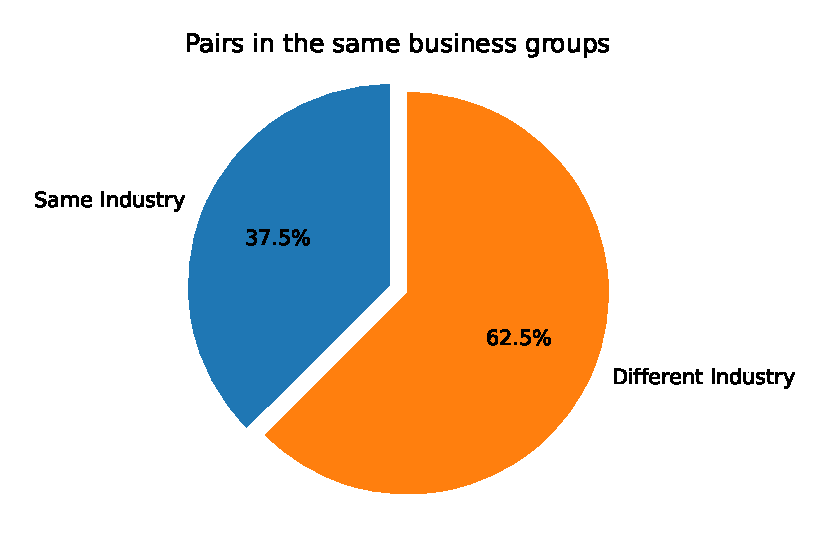
\includegraphics[width=0.48\linewidth]{Output/sameIndustryinBG.eps}
			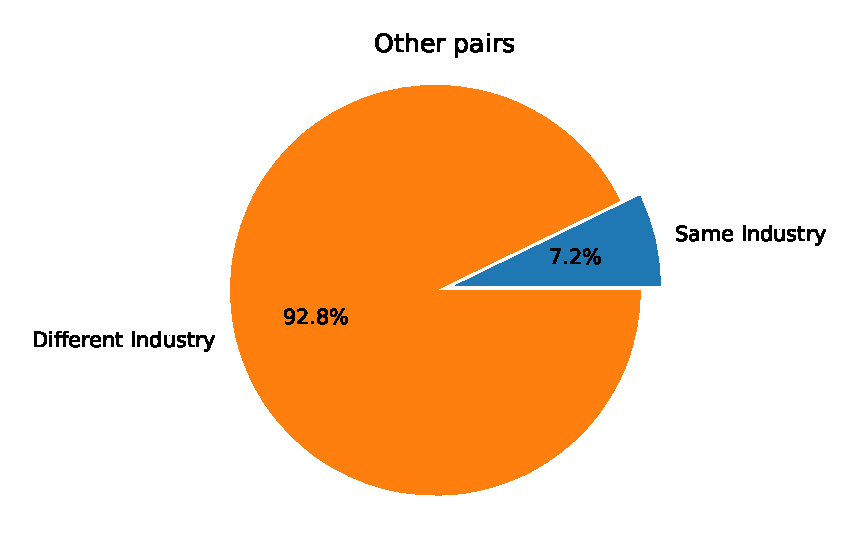
\includegraphics[width=0.48\linewidth]{Output/sameIndustryNoinBG.eps}
		\end{figure}
		\item 
		از نظر اندازه و نسبت بوک تو مارکت ججفت های گروه های کسب و کار شبیه جامعه هستند
		\item 
		همانطور که قبلا هم گفتیم متوسط مالکیت مشترک در گروه های کسب و کار زیاد است
		\item 
	شکل 
	\ref{BGSummary}
	خلاصه ها را نشان داده است
	\begin{figure}[htbp]
		\caption{}
		\label{BGSummary}
		\centering
		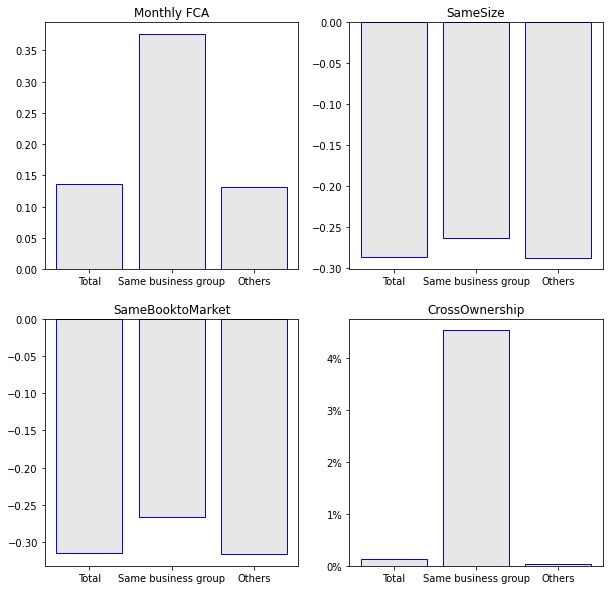
\includegraphics[width=0.85\linewidth]{Output/BGSummary.eps}
	\end{figure}
	\end{itemize}
	
	
\end{itemize}


\FloatBarrier





\end{appendices}

\end{document}